\chapter{Background} \label{sec:Background}

Simulations can only evaluate the effects of different control algorithms meaningfully if the underlying simulation models reasonably resemble reality. This background chapter provides an overview of the physical models used to describe the behavior of wind in Section~\ref{sec:Wind} and wind turbines in Section~\ref{sec:WindTurbines}. The interaction of wind turbines in farms via wake effects is described in Section~\ref{sec:WakeModels}. Baseline control schemes for both wind turbines and wind farms, against which the designs in this thesis are evaluated, are also presented in these sections. Section~\ref{sec:Control-Theoretic Background} presents the mathematical foundations of the two modeling frameworks used in this thesis, i.e., qLPV for wind turbines and Koopman for wind farms, followed by the MPC framework applied to both.

\section{Wind} \label{sec:Wind}

While wind, unlike conventional energy sources, cannot be controlled, its dynamics are well studied and understood. Detailed information on the aerodynamics of wind and wind turbines can be found, for example, in~\cite{hansen2015aerodynamics} and~\cite{hau20084}. The following section provides an overview of the related chapter in~\cite{Bianchi2007}, which summarizes the physics of wind.

Standardized wind models from the International Electrotechnical Commission (IEC) are used for testing and for the certification of controllers. The economic viability of a wind energy project, and hence decisions that need to be made prior to construction, such as number and exact location of turbines in a farm or turbine type, depend on the temporal and spatial wind distribution at the investigated site. These wind measurements also influence the choice of IEC wind models used for controller synthesis and closed-loop controller testing.

Wind is generated by temperature differences caused by uneven solar heating of the atmosphere. Wind can be classified into large-scale airflows, called geostrophic wind, which occurs in all layers of the atmosphere, and local wind. Local wind flows develop in the lower layer of the atmosphere, which extends up to a height of 100\,m and is therefore affected by geographical features and surface topography.

The kinetic energy frequency distribution of wind speeds follows a typical pattern, called the van der Hoven spectrum. The spectrum has two peaks, one at approximately 0.01 cycles per hour, representing a four-day cycle, and another at around 50 cycles per hour, roughly corresponding to one-minute cycles. These peaks are separated by an energy gap, indicating lesser energy content in wind speeds with frequencies between ten minutes and two hours. The low-frequency side of the spectrum is associated with geostrophic wind, while the high-frequency side represents local wind speeds, including turbulence. The aeroelastic forces that turbines are subjected to over their lifespan include mean wind speeds, i.e., constant stationary air movement, and stochastic turbulence. Hence, ten-minute time series with different mean values and different turbulence classes are traditionally used for controller testing and load analysis in wind energy applications.

The quasi-steady mean wind speed $\bar{V}$ at a site is the most important factor influencing the potential profitability of a wind energy project and the selection of appropriate wind turbines to maximize the annual energy production over the turbines' lifespan. The probability distribution of mean wind speeds is often predicted based on long-term measurements and can typically be approximated by the Weibull distribution:
\begin{equation}
    f_{\text{WB}}(\bar{V}) = \frac{k_{\text{WB}}}{C_{\text{WB}}}\left(\frac{\bar{V}}{C_{\text{WB}}}\right)^{k_{\text{WB}}-1}e^{- (\bar{V}/C_{\text{WB}})^{k_{\text{WB}}}}
\end{equation}
with shape and scale coefficients, $k_{\text{WB}}$ and $C_{\text{WB}}$, respectively, describing the probability of different wind speeds occurring at the site.

Mean wind speed also varies with height above ground level as surface roughness and obstacles affect wind speed through frictional forces. This spatial speed variation is called wind shear and can be described by different models, among them the exponential law:
\begin{equation}
    \bar{V}(z) =  \bar{V}(z_{\text{ref}})\left(\frac{z} {z_{\text{ref}} }\right)^{\alpha_{\text{shear}}} 
\end{equation}
where $z$ is the height above ground, $z_{\text{ref}}$ is a reference height, often 10\,m, and $\alpha_{\text{shear}}$ is the wind shear exponent. In \cite{Bianchi2007}, values for sand, mown and high grass, and suburban areas are given, varying from 0.10 to 0.32. In this work, the commonly used surface roughness exponent $\alpha_{\text{shear}} = 0.2$ is used.

While turbulence has a minor influence on Annual Energy Capture (AEC), it significantly impacts aerodynamic loads and power variance. Power variance is often called power quality, as maintaining a smooth power output is important, especially in smaller networks.

Turbulence is stochastically described by its power spectrum. Two widely used models are the von K\'arm\'an and Kaimal spectra:
\begin{equation}
    \Phi_{\text{K\'arm\'an}}(\omega) = \frac{K_V}{(1 +(\omega T_V)^2)^{5/6}} \quad \text{and} \quad \Phi_{\text{Kaimal}}(\omega) = \frac{K_V}{(1 +\omega T_V)^{5/3}}
\end{equation} 
where $\omega$ is the angular frequency, $T_V$ is the frequency bandwidth of the turbulence, and $K_V$ describes the turbulence power. For the von K\'arm\'an spectrum, they are approximated as:
\begin{equation}
    K_V = 0.475 I_v^2 \frac{L_v}{\bar{V}(z)} \quad \text{and} \quad T_V = \frac{L_v}{\bar{V}(z)}
\end{equation}
with the turbulence intensity $I_v$, which represents the ratio of the standard deviation of wind speed fluctuations to the mean wind speed, and the correlation length $L_v$, which indicates the scale of turbulence in space. The von K\'arm\'an model is implemented in the FASTTool, and therefore all the turbulent wind model test cases presented in this thesis leverage it.

The turbulence intensity, which depends on the height of the turbine and the terrain of a potential site, is an important factor in site selection. Higher turbulence intensity leads to increased aerodynamic loads on turbine structures, influencing the durability and performance of wind turbines.

\section{Wind Turbines} \label{sec:WindTurbines}

Wind turbines extract kinetic energy from the wind and convert it into other energy forms, most often electricity. In this section, commonly used mathematical representations based on the physics governing wind turbine behavior are provided, and a state-of-the-art control scheme for modern wind turbines is discussed.

\subsection{Wind Turbine Simulation Models}\label{windTurbineModel}
Depending on the application, different models are used to describe the physical effects of a wind turbine. In their simplest form, wind turbines can be modeled as an energy sink using the actuator disk model, which is the model used in WFSim~\cite{boersma2018control}. Alternatively, the Blade Element Momentum (BEM) model can be used directly, as in FAST~\cite{jonkman2005fast}, or via lookup tables for rotor thrust and torque to include the effect of varying rotor speed and pitch angles on the forces and moments. All models in this thesis are parameterized for the NREL 5MW reference 
turbine, with its physical parameters listed in Table~\ref{table:1}.

\subsubsection{Actuator Disk Model}
The amount of energy extracted from the wind depends on the wind speed difference between the wind in front of the turbine and the wind behind it. Figure~\ref{fig:ActDiscModel} visualizes the airflow through a rotor disk, showing the wind speeds, pressures, and corresponding areas of the airflow far ahead and far behind the turbine, as well as at the rotor.
%
\begin{figure}[ht]
    \center
    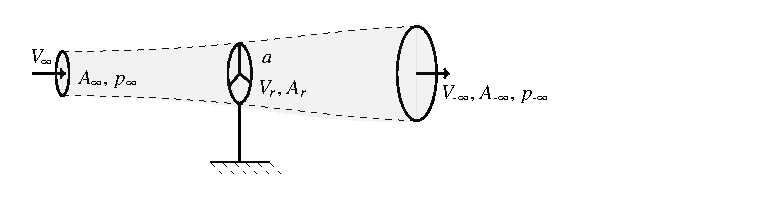
\includegraphics[width=0.76\textwidth,trim={0cm 0.3cm 3.5cm 0.4cm},clip]{figures/figuresBlockDiagram_IFAC23/testTurbineBetz.pdf}
    \caption{Airflow through a wind turbine, modelled as an actuator disk, adapted from \cite{Bianchi2007}.}
    \label{fig:ActDiscModel}
\end{figure}
%
The available amount of wind power $P_w$ and the amount of power $P_r$ extracted by the turbine rotor at the rotor area $A_r$ are given by:
\begin{eqnarray} \label{eq:PwPt}
    P_w = \frac{1}{2} \rho_a A_r V_{\infty}^3,\quad\text{and} \quad  P_r = c_P P_w,
\end{eqnarray}
where $\rho_a$ is the air density, $V_{\infty}$ is the freestream wind speed, and $c_P$ is the power coefficient. The ratio of freestream wind speed $V_{\infty}$ to the mean wind speed at the turbine rotor disk $V_r$, also called the effective wind speed, is:
\begin{eqnarray} \label{eq:ainduct}
    V_r = (1-a)V_{\infty},
\end{eqnarray}
where $a$ is the axial induction factor. The thrust $F_{T,r}$ acting on the turbine can be calculated from the pressure difference $\Delta p_r$ at the rotor disk. This pressure difference depends on the freestream wind and the recovered wind speed $V_{\text{-}\infty}$ far behind the turbines, leveraging Bernoulli's equation:
\begin{equation}\label{eq:pVBernoulli}
    \Delta p_r = \frac{1}{2} \rho_a(V_{\infty}^2  - V_{\text{-}\infty}^2 ).
\end{equation}
The thrust $F_{T,r}$ can be determined either from its rotor area and the pressure difference in Equation \eqref{eq:pVBernoulli}:
\begin{eqnarray} \label{eq:Ft1}
    F_{T,r} = A_r \Delta p_r =  \frac{1}{2} \rho_a A_r (V_{\infty}^2  - V_{\text{-}\infty}^2 ) 
\end{eqnarray}
or alternatively as the product of the air mass flow through the rotor area $\dot{m}_a$ and the wind speed difference:
\begin{eqnarray} \label{eq:Ft}
    F_{T,r} =  \dot{m}_a  (V_{\infty} - V_{-\infty}) = \rho_a A_r V_r (V_{\infty} - V_{\text{-}\infty}).  
\end{eqnarray}
From Equations \eqref{eq:ainduct}, \eqref{eq:Ft1}, and \eqref{eq:Ft}, the thrust of the rotor can be calculated as:
\begin{align} \label{eq:Ftall}
    F_{T,r} = 2a(1-a) \rho_a A_r V_{\infty}^2.
\end{align}
Combining Equations \eqref{eq:PwPt} to \eqref{eq:Ft} and using the fact that $P_r = F_{T,r} V_r$, the relationship between the axial induction factor $a$ and the power coefficient $c_P$ is:
\begin{equation}\label{eq:cpFromA}
    c_P(a) = 4a(1-a)^2,
\end{equation}
with the axial induction factor maximizing power yield given by $a^* = 1/3$ and the maximum $c_P(a^*) = 16/27$, known as the Betz limit. The wind speed difference and, consequently, the amount of power extracted from the wind, is influenced in real turbines by changing the generator speed and adjusting the blade pitch angle, both of which affect the turbine's rotor speed.

\subsubsection{Blade Element Momentum Theory}
The actuator disk model is a significantly simplified representation of the physics of a wind energy conversion system (WECS). Wind turbines consist of an aerodynamic subsystem, a flexible drivetrain, and a power generator, with the aerodynamic subsystem responsible for converting the available kinetic energy of the wind into useful mechanical energy through the rotor blades \cite{SaMuAlBe18}. 

Figure~\ref{figBEMModel} visualizes the local flow conditions and force components at a blade element, as used in Blade Element Momentum Theory (BEMT). In this model, the rotor is divided into small segments, each treated as an independent airfoil.
\begin{figure}[ht] %  %The Blade Element Momentum (BEM) model, as visualized in Figure \ref{figBEMModel}, refines the actuator disk model by incorporating the detailed aerodynamic behavior of individual rotor blades. 
    \center
    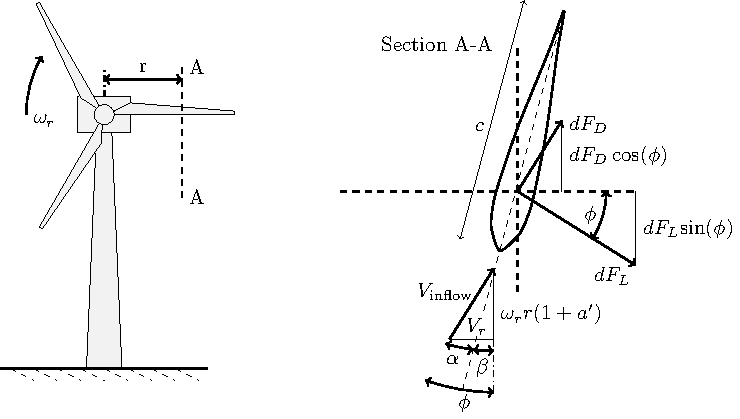
\includegraphics[width=0.96\textwidth,trim={0cm 0cm 0cm 0cm},clip]{figures/figuresBlockDiagram_IFAC23/turbineAirfoilBem.pdf}
    \caption{Local airflow and forces on a blade element of width $dr$ at radial position $r$, based on \cite{hansen2015aerodynamics} and adapted from \cite{weiss2016regelungstechnische}.} 
    \label{figBEMModel}
\end{figure}

BEMT combines the principles of blade element theory, which calculates the forces on each blade segment based on local airflow conditions, and momentum theory, which models the changes in wind velocity and pressure as air passes through the rotor disk. The lift and drag forces $dF_L$ and $dF_D$ on each blade element located at a radial position $r$ are determined by the angle of attack $\alpha$, the pitch angle $\beta$, the local airspeed $V_\text{inflow}$, the rotational speed of the rotor $\omega_r$, and the tangential flow induction factor $a^{\prime}$. The wind speed component $V_r$ is calculated from the freestream wind speed $V_{\infty}$ and the axial induction factor $a$ as described in Equation~\eqref{eq:ainduct}. The forces $dF_L$ and $dF_D$ are used to determine the thrust $F_{T,r}$ and torque $T_r$ generated by the rotor. 

The lift and drag forces, which act perpendicular and parallel to the inflow of a blade section with chord $c$ and width $dr$, are:
\begin{align} \label{eq:dFldFd}
    dF_L &= \frac{1}{2} \rho_a V^2_{\text{inflow}} c_L(\alpha)cdr,\\
    dF_D &= \frac{1}{2} \rho_a V^2_{\text{inflow}} c_D(\alpha)cdr,
\end{align}
where the lift and drag coefficients $c_L$ and $c_D$ depend on the angle of attack $\alpha$. As shown in Figure \ref{figBEMModel}, the angle $\phi$ between the local flow direction and the rotor plane is the sum of the angle of attack $\alpha$ and the pitch angle $\beta$. The thrust and torque of each segment can be calculated as:
\begin{align} \label{eq:dFTrdTr}
    dF_{T,r} &= dF_{L}\cos\phi + dF_D \sin\phi,\\
    dT_r &= (dF_{L} \sin \phi - dF_D \cos\phi) r.
\end{align}
The relative wind speed at the blade depends on its perpendicular and tangential components:
\begin{align} \label{eq:dFTrdTr1}
    V_{\text{inflow}} = V_{\infty}\sqrt{(1-a)^2 + \left(\frac{\omega_{r}r}{ V_{\infty}}(1+a^{\prime})\right)^2}\text{ and } \tan \phi = \frac{V_{\infty}}{\omega_r r} \frac{1-a}{1+a^{\prime}}.
\end{align} % where $a$ is the axial induction factor and $a^{\prime}$ is the tangential induction factor. 
The two induction factors $a$ and $a^{\prime}$ can be calculated if the blade element properties $c_L(\alpha)$, $c_D(\alpha)$, $r$, and $dr$ are known, as well as the current values of variables influencing the local force. These variables include $\rho_a$, $V_{\infty}$, $\omega_r$, and $\beta$. The BEM theory, as implemented in FAST, assumes steady, incompressible flow and calculates the rotor's performance iteratively using Equations \eqref{eq:pVBernoulli} to \eqref{eq:dFTrdTr1}. Thus, the interaction between the blade elements and the wind is considered in computing the forces, moments, and movements of the WECS. This iterative process is used to simulate performance under different wind conditions. The movement of the blades and tower is calculated in FAST using a linear modal representation, which leverages that the deflection angles are relatively small.

The wind turbine modeling approaches discussed in this section account for the influence of wind-speed variations on turbine operation. However, the instantaneous power extracted from the wind depends not only on the available wind speed but also on the turbine’s control inputs, generator speed, and blade pitch angle. The next subsection provides an overview of state-of-the-art wind turbine control strategies.


\subsection{Wind Turbine Control} \label{sec:WindTurbineControl}

All modern wind turbines use a control system to regulate rotor speed. The control settings of a wind turbine are determined by the energy available in the wind as well as economic considerations. Figure \ref{fig:WindREgion} visualizes the power output at different wind speeds.

\begin{figure}[ht]
\center
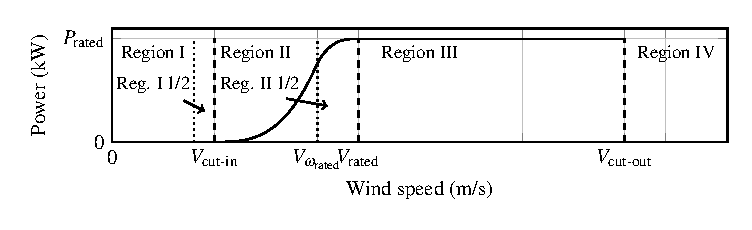
\includegraphics[width=0.8\textwidth,trim={0.5cm 0.4cm 0.0cm 0.3cm},clip]{figures/Figures_ADi/windRegionen.pdf}
\caption{Power output curve in Regions I to IV, based on the control region definitions for the NREL 5-MW reference turbine in \cite{jonkman2009definition}.}\label{fig:WindREgion}
\end{figure}

At very low wind speeds, below the so-called cut-in wind speed $V_{\text{cut-in}}$, the power that could be produced would not cover the operating costs. The wind speed region up to the cut-in wind speed is referred to as Region I. The wind speed region between the cut-in wind speed and the rated wind speed $V_{\text{rated}}$ of a turbine, i.e., the wind speed corresponding to the rated power of the turbine, is called Region~II. 

For wind speeds above the rated wind speed, the blades are pitched to keep the power output constant and to reduce excessive mechanical loads that would otherwise shorten the turbine's operational lifespan. At very high wind speeds, above the cut-out wind speed $V_{\text{cut-out}}$, the turbine stops operating. Region III is the wind speed range between rated and cut-out wind speed, while Region IV refers to wind speeds above the cut-out wind speed.

At each wind speed between the cut-in and cut-out wind speeds, a control system ensures the most profitable power output by regulating the generator torque $T_g$ and the blade pitch angle $\beta$. Generator torque is used to maximize power yield at wind speeds in Region~II. The blade pitch is used to maintain a constant power output at rated power for wind speeds above the rated wind speed and below the cut-out wind speed in Region~III. The power controller receives feedback from the generator rotational speed $\omega_g$ across all operating regions. 

In this work, the power controller available within TU Delft's FASTTool \cite{mulders2020wind} is used as a baseline, see Table~\ref{table:pitch_ctrl} for its parameters. FASTTool features a MATLAB graphical user interface for setting up simulations and tuning control parameters for an underlying Simulink model, which represents the dynamics of the NREL 5MW turbine. The underlying physical principles are detailed in \cite{jonkman2009definition}. 


\subsubsection{Generator Torque Control}

In Regions I\,1/2 and II, the generator torque is governed by the so-called $k\omega^2$ control law, which is implemented as a tabulated function of the generator speed $\omega_g$. In Region~I\,1/2, the start-up phase just below the cut-in wind speed, see Figure~\ref{fig:WindREgion}, a multiplication factor is applied to compute the reference generator torque $T_{g,\text{ref}}$. In most of Region~II, an optimal factor $K^*$ is multiplied by the square of the rotational speed.

The upper portion of Region II, just below the rated wind speed, is referred to as Region~II\,1/2. In this transition zone, a smooth linear interpolation is applied up to the rated rotational speed. This ensures a seamless transition within Region~II while also maintaining compliance with noise emission regulations and limiting excessive mechanical loads. These controller settings, originally defined in \cite{jonkman2009definition}, have been implemented without modifications in \cite{mulders2020wind}, preserving both the algorithmic structure and parameter values.

\subsubsection{Blade Pitch Control} 

In Region III, the collective pitch control strategy relies on a scheduled proportional-integral (PI) controller, where the proportional and integral gains, $K_P(\omega_g)$ and $K_I(\omega_g)$, are dynamically adjusted based on the generator speed. This adaptive gain scheduling enhances the tracking of the maximum allowable rotor speed. The gain values used in this implementation remain unchanged from those provided in the original FASTTool repository.

The derivation of these gains follows from \cite{jonkman2009definition}. The difference between the aerodynamic torque $T_r$ and the generator torque $T_g$, with the latter multiplied by the gear ratio $N_g$, is equal to the product of drivetrain inertia $J_{s}$ and the rotor acceleration $\Delta \dot{\omega}_r$:

\begin{equation} \label{eq:Tr1_background}
T_r -N_g T_g = (J_r + N_g^2 J_g) \frac{d}{dt}(\omega_{\text{rated}} + \Delta \omega_r) = J_{s} \Delta \dot{\omega}_r,
\end{equation}
where $J_r$ and $J_g$ are the rotor and generator inertias, respectively. The aerodynamic and generator torques, derived from the rated power $P_{\text{rated}}$, can be approximated as Taylor series expansions:

\begin{eqnarray}
T_g(\omega_r) &=& \frac{P_{\text{rated}}}{N_g \omega_r} \approx  \frac{P_{\text{rated}}}{N_g \omega_{\text{rated}}} - \frac{P_{\text{rated}}}{N_g\omega_{\text{rated}}^2} \Delta \omega_r,  \label{eq:Tg}\\
T_r(\beta) &=& \frac{P(\beta,\omega_r)}{\omega_r}   \approx \frac{P_{\text{rated}}}{\omega_{\text{rated}}} + \frac{1}{\omega_{\text{rated}}}\Big(\frac{\partial P}{\partial \beta}\Big) \Delta \beta.  \label{eq:Tr_background}
\end{eqnarray}
%
The desired change in pitch angle, $\Delta \beta$, is calculated based on the rotor speed deviation $\Delta \omega_r$ using a proportional-integral-derivative (PID) controller:

\begin{eqnarray} \label{eq:PID}
\Delta \beta = K_P N_g \Delta \omega_r + K_I \int_{0}^{t}N_g \Delta \omega_r dt + K_D N_g \Delta \dot{\omega}_r.
\end{eqnarray}
%
Substituting Equation~\eqref{eq:PID} into Equation~\eqref{eq:Tr_background} and incorporating the relationships from Equations \eqref{eq:Tr1_background} and \eqref{eq:Tg} leads to the final control formulation with the substitute state $\dot{x} = \Delta \omega_r$ and derivative $\mathcal{P}_\beta = \left( -\frac{\partial P}{\partial \beta} \right)$:

\begin{equation}\label{eq:PID2} 
\underbrace{\left[ J_{s} + \frac{\mathcal{P}_\beta}{\omega_{\text{rated}}} N_{g} K_D \right]}_{M_{x}} \ddot{x}(t) 
+ \underbrace{\left[ \frac{\mathcal{P}_\beta}{\omega_{\text{rated}}} N_{g} K_P - \frac{P_{\text{rated}}}{\omega_{\text{rated}}^2} \right]}_{C_{x}} \dot{x} (t)
+ \underbrace{\left[ \frac{\mathcal{P}_\beta}{\omega_{\text{rated}}} N_{g} K_I \right]}_{K_{x}} x(t) = 0.
\end{equation}
%
The PID gains are determined to achieve the desired natural frequency and damping ratio, which, in turn, dictate how the mass $M_{x}$, damping $C_{x}$, and spring term $K_{x}$ should be set through the control parameters. The value of  $\mathcal{P}_\beta$, i.e., the sensitivity of the aerodynamic power to the blade pitch, can be calculated for the different operating points and is provided in \cite{jonkman2009definition}. 

In the implementation of \cite{mulders2020wind}, a gain-scheduled PI controller is used by default, with the derivative term set to zero. The controller gains are modified from those originally suggested in \cite{jonkman2009definition}, aiming to achieve a smoother power output. A fixed-gain PI controller is also available in FASTTool, but for this study, the default gain-scheduled PI controller is employed.

\subsubsection{Yaw Control}
Yaw control in modern wind turbines is responsible for aligning the turbine with the wind direction based on measurements from anemometers mounted on the nacelle. The mean wind speed is assessed over ten-minute intervals, and yaw adjustments are performed at the same interval if the yaw misalignment exceeds a predefined threshold. Due to the large structural loads associated with yaw motion, adjustments are made infrequently to ensure the longevity of the yaw system. As a result, yaw control does not directly influence the turbine's power control.

However, in wind farm settings, deliberate yaw misalignment, i.e., intentional yaw offset, has been actively researched over the past decade as a means to mitigate wake effects on downstream turbines. By strategically redirecting the wake, this approach aims to optimize the overall power output of a wind farm rather than maximizing the efficiency of individual turbines.

\subsection{Control Objectives}\label{subsection Control Objectives}
The overall goal of both wind turbine and wind farm control is to minimize the levelized cost of energy (LCoE). This requires balancing the often contradictory objectives of maximizing power yield while minimizing mechanical damage equivalent loads (DEL) on the tower and blades, as well as reducing actuator energy consumption. Below is a brief overview of load analysis for wind turbine controllers and the objectives for controller evaluation applied in this thesis. The five criteria described below are taken from \cite{hoffmann2018load}.

\subsubsection{Load Analysis}
Before wind turbine controllers are applied in production, they must be certified based on an extensive load analysis. This analysis uses Design Load Cases (DLCs), which are 22 standard scenarios defined by the IEC61400-1~\cite{IEC61400-1} and classified into 17 ultimate and 5 fatigue load case scenarios. The selection of DLCs used for load analysis depends on the mean wind speed at the location of the WECS, which influences the decision on whether Class I, II, or III turbines are chosen. The average wind speeds for these turbine classes are 10\,m/s, 8.5\,m/s, and 7.5\,m/s, respectively. In addition to the mean wind speed, turbulence intensity is also considered, with three different classes. In this work, the turbulence intensity values for IEC Classes A, B, and C are used as implemented in the \textit{InflowWind.m} file of the FASTTool, which are 16\%, 14\%, and 12\%, respectively. These values reflect the state of the software tool at the time of writing and may differ from those defined in the latest IEC 61400-1 standard or from other literature: For example, according to \cite{gasch2011wind} Class A corresponds to a turbulence intensity of 18\% and Class B to 16\%.

The ultimate load DLCs are used to verify that a turbine can withstand the maximum load that is statistically likely to occur during its lifetime. Fatigue load analysis is applied to demonstrate that a turbine can endure structural loads over time. For this analysis, closed-loop simulations of 660\,s are conducted using different turbulent wind test cases from the relevant IEC wind classes, with different random seeds for wind initialization. The first 60\,s of simulated data are discarded to avoid introducing initialization artifacts into the analysis, and the remaining 600\,s are used to calculate the DEL. This approach is used in the context of certification to verify the suitability of a control strategy. In this thesis, it is applied for controller testing and performance comparison.

\subsubsection{DEL Criteria $C_{\text{DEL},b}$ and $C_{\text{DEL},t}$}

For the DEL calculation of signals such as blade and tower bending moments, their load cycles are first classified using rainflow counting \cite{matsuishi1968fatigue}. In this thesis, the MATLAB implementation in \textit{rainflow.m} is used to derive the cycle count vector $\bm{l}_D \in \mathbb{R}^{n_l \times 1}$ and their respective range vector $\bm{R}_{\text{DEL}}\in \mathbb{R}^{n_l \times 1}$, i.e., their peak-to-peak amplitudes, for the simulation signal of a bending moment, with $n_l$ as the number of stress levels. 

In a second step, the elements of the vectors $\bm{l}_D$ and $\bm{R}_{\text{DEL}}$ are applied to calculate damage from the moment signals. This is based on Miner’s rule, which calculates damage from stress signals as:
\begin{equation} \label{eq:Miner0}
D =  \sum_{i=1}^{n_l} D_i = \sum_{i=1}^{n_l} \frac{l_i}{L_i} = 
\sum_{i=1}^{n_l} \left( \frac{l_i}{L_D} \left(\frac{\sigma_i}{\sigma_D} \right)^m \right)
= \frac{1}{L_D\sigma_D^m} \sum_{i=1}^{n_l}  \left( l_i \sigma_i^m \right)
\end{equation}
where $D$ represents the damage fraction at a given point in time, with $D = 1$ indicating the end of the remaining useful life. The mean number of cycles to failure is denoted $L_i$, and $l_i$ is the recorded number of cycles at stress level $\sigma_i$. The equation can be reformulated to explicitly account for material properties, where $L_D$ is the terminal load at that stress level, $\sigma_D$ and $\sigma_i$ are the terminal and actual occurring stress amplitudes, respectively, and $m$ is the Woehler coefficient, which depends on the material. In this thesis, the commonly used Woehler coefficients of $m_{\text{Steel}} = 4$ for the tower and $m_{\text{GFRP}} = 10$ for the blades of the NREL 5MW, which are made of glass fiber reinforced polymer (GFRP), are used.

Leveraging Equation~\ref{eq:Miner0}, a reference range $R_{\text{DEL},\text{ref}}$ and reference cycle number $l_{\text{ref}}$ are introduced:
\begin{eqnarray}
l_{\text{ref}} R_{\text{DEL},\text{ref}} ^m = \sum_{i=1}^{n_l}  \left(l_i R_{\text{DEL},i}^m \right) \iff R_{\text{DEL},\text{ref}} = \sqrt[m]{\frac{ \sum_{i=1}^{n_l} \left(l_i R_{\text{DEL},i}^m \right)}{l_{\text{ref}}}}.
\end{eqnarray}
The reference number of cycles is set to the commonly used value $l_{\text{ref}}=2\cdot10^6$. From the reference range, the DEL over the lifetime can be derived by calculating the reference range for the different wind speed and turbulence scenarios likely to occur and weighting them using Weibull distributions.

In this thesis, reference numbers for the blade and tower DELs, $R_{\text{DEL},b,\text{Ref}}$ and $R_{\text{DEL},t,\text{Ref}}$, respectively, are calculated for a closed-loop simulation run with the baseline controller, as described in Section \ref{sec:WindTurbineControl}. A second simulation with the same wind file is then run with the controller design to be compared with this baseline, e.g., a qLMPC design. The resulting damage numbers for this run are divided by the baseline numbers to form the criteria $C_{\text{DEL},b}$ and $C_{\text{DEL},t}$. Values below 1 hence indicate a reduction in blade and tower loads, respectively, and are therefore considered an improvement of the closed-loop behavior.

\subsubsection{Power Reference Tracking and Standard Deviation Criteria $C_{\bar{P}}$ and $C_{\delta P}$}

Another performance criterion in wind turbine control is the power reference tracking error, which should not exceed that of the baseline control case. The standard deviation of power output is also used as a metric. Particularly in smaller networks, a stable power output, i.e., a power output with a small standard deviation, affects grid stability by reducing fluctuations. The objectives $C_{\bar{P}}$ and $C_{\delta P}$ are calculated by normalizing the values obtained from simulations with the controller designs developed in this work by the values obtained from simulations with the baseline controller.

\subsubsection{Pitch Actuator Energy Criterion $C_{\Delta\beta}$}

Actuator movements must be limited to prevent excessive wear of the mechanical pitch actuators and avoid unnecessary energy consumption. The calculation of actuator power considers the change in blade pitch angles and multiplies them by the pitching moment of the same blade. Like the other objectives, the criterion $C_{\Delta\beta}$, which is the product of the pitch angle derivative and pitching moment obtained with the newly designed controller, is divided by the same product from a simulation run with the baseline controller.

The equations and numerical evaluations of all objectives are presented in Chapter~4, where these metrics are used for the performance assessment of a qLMPC, a PID-IPC, and a PID-AALC design for the NREL 5MW turbine.


\section{Wind Farms}\label{sec:WakeModels}

Wind turbines are grouped into farms to maximize energy yield within the available land or offshore space while minimizing operational and maintenance costs. However, wake interactions between turbines lead to power losses and introduce additional mechanical loads on downstream turbines. While the current state-of-the-art farm control primarily sets the power demands for individual turbines, numerous studies, including field tests, have demonstrated the advantages of coordinated wind farm control in both load reduction and power maximization \cite{houck2022review}.

Understanding how turbines interact aerodynamically within a farm is essential for designing an effective control strategy. Accurately modeling wind turbine wakes has been a significant research focus over the past four decades. The choice of wake model depends on the required trade-off between computational efficiency and accuracy. Typically, low- to medium-fidelity models are used for controller synthesis, while medium- to high-fidelity models are preferred for controller evaluation.

This section provides an overview of different wake modeling approaches, including their underlying physical principles and software implementations. The Jensen Park model \cite{jensen1983note} is presented for completeness, as it demonstrates that cooperative wind farm control can yield increased power. The Bastankhah Gaussian wake model \cite{bastankhah2016experimental} is used in Chapter 5 for calculating the optimal yaw settings. The Navier-Stokes Equations (NSE) are discussed in detail, as they are used in linearized form in WFSim. Additionally, a section on wind farm control, as implemented in WFSim, is included.


\subsection{Wind Farm Simulation Models and Environments}\label{Subsection:WindFarmSimulationModels}

Table \ref{tab:WFModels} provides an overview of analytical wind farm models and software used to simulate wind farm behavior. It is adapted with minor modifications and additions from the thesis \cite{smits2023fast}. The models and software utilized in this work are marked in bold. The computational effort for the medium- to high-fidelity models is given with respect to the ten-minutes wind signals used for load analysis. Low-fidelity models are commonly used to account for the decrease in power production due to wakes in annual energy production (AEP) calculations for wind farms. These models are essential for layout optimization and for generating lookup tables for static yaw misalignment control. 

\begin{table}[ht]
\begin{center}
\resizebox{\textwidth}{!}{
\begin{tabular}{p{3cm} p{2cm} p{3cm} p{2cm} p{3cm}}
    \toprule
    Analytical Model/Software & Language & Flow Type & Fidelity & Computational Effort\\
    \midrule
    Jensen Park &  & \multirow{3}{3cm}{Static 2D parametric} & \multirow{3}{2cm}{Low} & \multirow{3}{3cm}{Seconds}\\
    Frandsen & Analytic &  &  & \\
    \textbf{Bastankhah Gaussian} &  &  &  & \\
    \midrule
    FLORIS & Python & \multirow{2}{3cm}{Static/Dynamic 2D parametric} & \multirow{2}{2cm}{Low to medium} & \multirow{2}{3cm}{Seconds to minutes}\\
    FLORIDyn & MATLAB &  &  & \\
    \midrule
    \textbf{WFSim} & MATLAB & 2D-NSE & \multirow{2}{2cm}{Medium} & \multirow{2}{3cm}{Minutes to Hours}\\
    FAST.Farm & Fortran & DWM/3D-NSE &  & \\
    \midrule
    SOWFA  &  \multirow{3}{2cm}{Fortran} & \multirow{3}{2cm}{LES/3D-NSE} & \multirow{3}{2cm}{High} & \multirow{3}{3cm}{Hours to days}\\
    PALM & & & &\\
    EULAG  & & &  &\\
    \bottomrule
\end{tabular}
}
\caption{Overview of wind farm models and simulation tools. Models and software marked in bold are used in this thesis.}
\label{tab:WFModels}
\end{center}
\end{table}

The Jensen Park model, based on mass conservation and the actuator disk model, is widely used for turbines aligned with the main wind direction, meaning turbines without yaw misalignment. Originally proposed by \cite{jensen1983note}, this model assumes a linearly expanding wake with a velocity deficit that depends solely on the distance behind the rotor. This so-called "top-hat" model simplifies calculations and remains relevant for layout optimization and power estimation. 

The Frandsen model \cite{frandsen2006analytical}, a more recent parametric model, builds upon mass and momentum conservation principles. Unlike the Jensen Park model, the Frandsen model introduces a "tube" concept for near-wake modeling and uses a different approach for merging multiple wakes. Both models have been extended to incorporate Gaussian wake distributions, as studies have shown that Gaussian profiles better match high-fidelity simulations \cite{sizhuang2014analysis} and experimental measurements \cite{chen2020data}.

A widely used closed-form analytical model for wake-induced wind speed deficits, developed and validated against wind tunnel data in \cite{bastankhah2016experimental}, is particularly useful for modeling wake redirection effects due to yaw misalignment. This model has been applied in research on combined axial induction and wake redirection control strategies \cite{boersma2019constrained} and is implemented in the software FLOw Redirection and Induction in Steady-State (FLORIS) \cite{fleming2021experimental}.

FLORIS provides a range of wake models with varying fidelity levels, including analytical models with and without Gaussian wake profiles, as well as the curl model, which accounts for wake asymmetries. FLORIDyn \cite{becker2022FLORIDyn} is a MATLAB-based adaptation of FLORIS designed for evaluating controller performance. WFSim, also MATLAB-based, uses a linearized two-dimensional NSE to model flow dynamics while employing the actuator disk model for turbine behavior. FAST.Farm \cite{jonkman2017development} calculates flow using the dynamic wake model (DWM) and turbine dynamics using BEM theory (BEMT).

Higher-fidelity models implemented in Computational Fluid Dynamics (CFD) software, such as SOWFA \cite{fleming2014evaluating}, PALM \cite{maronga2015parallelized}, and EULAG \cite{prusa2008eulag}, employ large eddy simulation (LES) techniques in order to solve the three-dimensional NSEs which model wind farm flow. LES is a computational fluid dynamics technique that resolves the large, energy-containing turbulent structures directly while modeling the effects of smaller, subgrid-scale eddies. This provides high-fidelity predictions of turbulent flow at a lower computational cost than direct numerical simulation. Despite this reduction, the computational costs of LES remain relatively high, and CFD codes are typically run on server clusters with tens of cores, often requiring hours to days to simulate realistic wind farm scenarios.

Given these high computational costs, simplified engineering wake models provide a practical alternative for rapid wind farm analysis and control design. These models approximate turbine wakes using analytical formulations, allowing for fast simulations while capturing the essential flow effects. The following subsections introduce representative models of varying complexity, starting with the Jensen Park and Bastankhah Gaussian wake models, and concluding with the NSE-based approach implemented in WFSim.

\subsubsection{Jensen Park Model for Turbines without Yaw Misalignment} \label{subsecJensen}
The Jensen Park model, based on the conservation of mass and the actuator disk model, is used for turbines aligned with the main wind direction, i.e., turbines without yaw misalignment. First proposed in \cite{jensen1983note}, it is still widely used due to its simplicity, not only for AEP calculations but also in scientific studies. For example, \cite{barreiro2019data}, from which the equations below are taken, uses it to demonstrate the applicability of game theory to wind farm control. 

According to \cite{jensen1983note}, the power $P_i$ of the $i^{\text{th}}$ turbine in a wind farm with $n_{\text{WT}}$ turbines is given by:
\begin{align}\label{eqPAIC}
P_{i} (\bm{a}_i) &= \frac{1}{2} \rho_a A_{ri} c_{P}(a_{i}) V_{i}^3(\bm{a}_{i-1}),
\end{align}
where $\rho_a$ is the air density, $A_{ri}$ is the rotor surface area, $c_P$ is the power coefficient, $V_{i}$ is the wind speed at turbine $i$, and $a_i$ is the axial induction factor. The vector $\bm{a}_{i-1} \in {\mathbb{R}}^{i-1}$ represents the axial induction factors of all upstream turbines of the $i^\text{th}$ turbine, while $\bm{a}_{i} \in {\mathbb{R}}^{i}$ is a concatenation of $\bm{a}_{i-1}$ and $a_i$.

The power coefficient $c_{P,i}$ depends on the axial induction factor $a_i$, as defined in Equation~\eqref{eq:cpFromA}:
\begin{align} \label{eqcP_from_a}
c_{P,i}(a_i) &= 4a_i(1-a_i)^2.
\end{align}
%
The wind speed $V_{i}$ at turbine $i$ depends on the freestream wind speed $V_\infty$, the axial induction of all upstream turbines, i.e., all turbines in the set $\mathcal{W} = \{1,2,...,j,...,i,... n_{\text{WT}}\}$, and the coefficient $c_{ji}$:
\begin{align} \label{eqVri}
V_{i}(\bm{a}_{i-1}) &= V_\infty \left( 1 - 2\sqrt{\sum \limits_{j\in \mathcal{W}, \bm{x}_i>\bm{x}_{j}} (a_{j} c_{ji})^2} \right),
\end{align}
which depends on the rotor diameter $D_{rj}$, turbine position $x_i$, and wake expansion coefficient $b$:
\begin{align*}
c_{ji} &= \left(\frac{D_{rj}}{D_{rj} + 2b (x_i - x_{j})}\right)^2,
\end{align*} with $b = 0.075$, a typical value for onshore turbines. 

Figure \ref{figWindfarmAIC} visualizes the wind farm setup used for axial induction control (AIC) design for NREL 5MW turbines spaced five times their rotor diameter apart.

\begin{figure}[ht]
\center
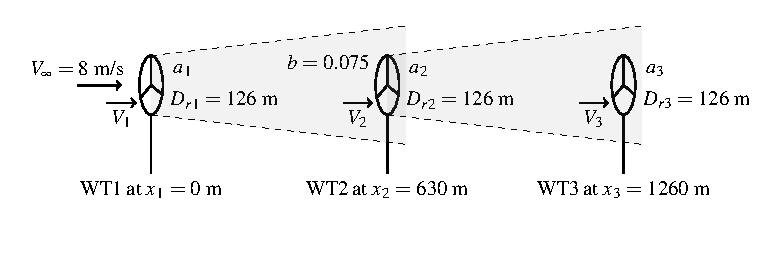
\includegraphics[width=0.8\textwidth,trim={0.5cm 1.3cm 0.2cm 0.3cm},clip]{figures/figDirETC/testAICPark.pdf}
\caption{Schematic visualization of AIC wind farm optimization, adapted from \cite{barreiro2019data}.}
\label{figWindfarmAIC}
\end{figure}
%
The farm power $P_{\text{WF}}(\bm{a_{n_{\text{WT}}}})=\sum\limits_{i=1}^{n_{\text{WT}}}P_i(a_i)$ can be optimized by adjusting the axial induction factors of all turbines. This is done by inserting Equations~\eqref{eqcP_from_a} and \eqref{eqVri} into Equation~\eqref{eqPAIC}. 

Note that the Jensen model assumes all turbines are facing the wind and is therefore not suitable for calculating wake effects of turbines with intentional yaw misalignment, as used in wake redirection control (WRC). For this, the Bastankhah Gaussian wake model is used.

\subsubsection{Bastankhah Gaussian Model for Turbines with Yaw Misalignment}\label{secBastankhah}
In static Wake Redirection Control (WRC), the wake is steered away from downstream turbines by tilting or yawing the upstream turbines \cite{fleming14wakeeval}. A widely used analytical closed-form model for the wind speed deficits of a downstream turbine was developed and validated against wind tunnel data in \cite{bastankhah2016experimental}. The equations from this study are provided below for completeness.

Figure \ref{figWindfarmWRC} provides a two-dimensional schematic plot of the three-dimensional WRC setup for an array of three turbines.
%
\begin{figure}[ht]
\center
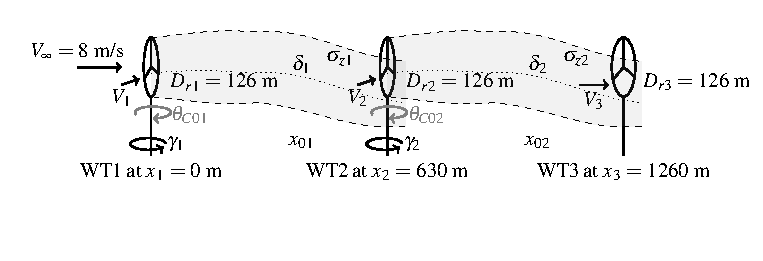
\includegraphics[width=0.8\textwidth,trim={0.5cm 1.3cm 0.2cm 0.3cm},clip]{figures/figDirETC/testWRCGaussiank.pdf}
\caption{Schematic visualization of WRC wind farm optimization, adapted from \cite{bastankhah2016experimental}.}
\label{figWindfarmWRC}
\end{figure}
%
The wake angle at the rotor, $\theta_{C0i}$, and the beginning of the far-wake region, $x_{0i}$, for which the model is shown to yield accurate results, are calculated using the approximation of the thrust coefficient $c_T$ from the axial induction factor $a_i$ and turbine yaw angle $\gamma_i$:
\[
c_T \approx 4a_i(1-a_i\cos(\gamma_i)).
\]
The wake angle $\theta_{C0i}$ at the rotor is given by:
\[
\theta_{C0i} =\frac{0.3\gamma_i}{\cos(\gamma_i)}(1-\sqrt{1-c_T\cos(\gamma_i) }).
\]
The start of the far-wake region $x_{0i}$ is computed as:
\[
\frac{x_{0i} }{D_r}=\frac{\cos(\gamma_i)(1+\sqrt{1-c_T })}{\sqrt{2}\left\lbrack k_{\alpha^*} I_i + k_{\beta^*} (1-\sqrt{1-c_T })\right\rbrack } 
\]
with coefficients $k_{\alpha^*}= 2.32 $ and $k_{\beta^*} = 0.154$ from \cite{bastankhah2016experimental}. The local turbulence intensity at hub height $z_h$ in front of the turbine, $I_i$, is defined as the ratio of wind speed fluctuations to the mean wind speed.
The wake deflection centerline $\delta_i$ for the far-wake region with $x > x_{0i}$ is given as:
\[
\frac{\delta_i}{D_r} =\theta_{C0i} \frac{x_{0i}}{D_r}  + \frac{\theta_{C0i}}{14.7} \sqrt{\frac{\cos(\gamma_i)}{b_y b_z c_T}} (2.9 +1.3\sqrt{1-c_T}-c_T)K_{\text{ln}}
\]
with:
\[
K_{\text{ln}}= \ln\left( \frac{(1+\sqrt{c_T })(1.6\sqrt{\frac{8\sigma_{yi}\sigma_{zi}}{D_r^{2} \cos(\gamma_i)}}-\sqrt{c_T })}{(1-\sqrt{c_T })(1.6\sqrt{\frac{8{\sigma_{yi} \sigma_{zi}}}{D_r^{2} \cos(\gamma_i) }}+\sqrt{c_T })} \right)
\]
and wake expansion coefficients $b_y$ and $b_z$ for lateral and vertical wake expansions. The wake expansions $\sigma_{yi}$ and $\sigma_{zi}$ are:
\[
\frac{\sigma_{yi} }{D_r}=b_y \frac{(x-x_{0i} )}{D_r}+\frac{\cos(\gamma_i)}{\sqrt{8}}, \quad
\frac{\sigma_{zi}}{D_r}=b_z\frac{(x-x_{0i} )}{D_r}+\frac{1}{\sqrt{8}}.
\]
The far-wake velocity deficit, and consequently the wind speed at a downstream turbine, is calculated using the Gaussian wake model:
\[
V_i = V_{i-1}(1 - (1- K_C)e^{-0.5((y-\delta_i)/\sigma_{yi})^2} e^{-0.5((z-z_h)/\sigma_{zi})^2})
\]
where:
\[
K_C = \sqrt{1-\frac{c_T \cos(\gamma_i)}{8(\sigma_{yi} \sigma_{zi}/D_r^2)}}
\]
and $V_0 = V_{\infty}$, meaning that for the first turbine, $V_1 = V_{\infty}$ due to the freestream wind acting on it, resulting in $K_C= 1$.
The turbine power output is then calculated as:
\[
P_i(\bm{a}_i,\bm{\gamma}_i) = \frac{1}{2} \rho_A A_r c_{P}(a_i,\gamma_i)(V_{i}(\bm{a}_{i-1},\bm{\gamma}_{i-1}) \cos(\gamma_i))^3
\]
where the power coefficient $c_P$ is given by:
\[
c_P(a_i,\gamma_i)  \approx 4a_i(1-a_i\cos(\gamma_i))^2.
\]
%
The results from the Gaussian wake model are compared to those obtained from $\text{WFSim}$, which is based on a linearized form of the $\text{Navier-Stokes equations (NSE)}$. While the Gaussian model offers computational speed, it relies on empirical parameters and cannot capture complex, dynamic flow phenomena like wake-wake interaction or pressure effects. Therefore, to achieve higher fidelity while maintaining a feasible computational cost for control design, the simulation environment $\text{WFSim}$ is employed. An overview of the control-oriented $\text{NSEs}$ on which this simulator is based is provided in the next subsection.

\subsubsection{Navier-Stokes Equations (NSE)}
The fluid dynamics of the turbine wake, affecting air pressure and wind speed, are fundamentally described by the NSE. In their two-dimensional, incompressible form, considering only the longitudinal and lateral velocity components and neglecting the vertical component, the equations governing the momentum and mass conservation are given as \cite{boersma2018control}:
\begin{align*}
\underbrace{
\begin{bmatrix}
\frac{\partial v_x}{\partial t} \\[1mm]
\frac{\partial v_y}{\partial t}
\end{bmatrix}
}_{\text{local acceleration}}
+
\underbrace{
\begin{bmatrix}
v_x \frac{\partial v_x}{\partial x} + v_y \frac{\partial v_x}{\partial y} \\[1mm]
v_x \frac{\partial v_y}{\partial x} + v_y \frac{\partial v_y}{\partial y}
\end{bmatrix}
}_{\text{convective term}}
+
\underbrace{
\begin{bmatrix}
\frac{\partial p}{\partial x} \\[1mm]
\frac{\partial p}{\partial y}
\end{bmatrix}
}_{\text{pressure gradient}}
+
\underbrace{
\begin{bmatrix}
\frac{\partial \tau_{xx}}{\partial x} + \frac{\partial \tau_{xy}}{\partial y} \\[1mm]
\frac{\partial \tau_{yx}}{\partial x} + \frac{\partial \tau_{yy}}{\partial y}
\end{bmatrix}
}_{\text{subgrid stress divergence}}
-
\underbrace{
\begin{bmatrix}
f_x \\[1mm]
f_y
\end{bmatrix}
}_{\text{turbine forcing}}
&= 
\begin{bmatrix} 0 \\ 0 \end{bmatrix}, \\[2mm]
\underbrace{\frac{\partial v_x}{\partial x} + \frac{\partial v_y}{\partial y}}_{\text{mass conservation / incompressibility}} &=   -\frac{\partial v_y}{\partial y}
\end{align*}
with $v_x$ and $v_y$ as wind components in the longitudinal $x$ and lateral $y$ directions, respectively, air pressure $p$, stress components $\tau_{xx}$, $\tau_{xy}$, $\tau_{yx}$ and $\tau_{yy}$, and turbine thrust $f_x$ and $f_y$. The four subgrid stress components $\tau_{ij}$ are the normal and shear stresses, where the first index indicates the direction of the momentum affected and the second index is the direction of the gradient causing the stress. The seemingly counter-intuitive second equation arises because the model must account for air passing over the turbine area rather than being forced to entirely circumvent it. The dimension reduction from the 3D equations, where longitudinal, lateral, and vertical velocity gradients sum to zero, is modeled in \cite{boersma2018control} via the approximation $\partial v_y/\partial y = \partial v_z/\partial z$. This approximation enables WFSim to avoid the so called blockage-effect typical of 2D models.
%
For compactness, these equations can be expressed in vector form as
\begin{align} \label{eq:NSE2d}
\frac{\partial \bm{v}}{\partial t}+ (\bm{v}\cdot \nabla_H)\bm{v} + \nabla_H p + \nabla_H\cdot\bm{\tau}_h  - \bm{f} = \bm{0}_{2\times1},\quad  
\nabla_H\cdot \bm{v} = -\frac{\partial v_y}{\partial y}
\end{align}
where:
\begin{itemize}
\item $\bm{v} =[v_x\;\;v_y]^T$ represents the wind speed vector.
\item The term $\frac{\partial \bm{v}}{\partial t}$ denotes the local acceleration of the wind flow over time.
\item The term $\nabla_H = [\frac{\partial}{\partial x}\;\;\frac{\partial}{\partial y}]^T$ is the gradient operator in the 2D simulation plane. Thus, the convective term $(\bm{v}\cdot \nabla_H)\bm{v}$ is the advection of momentum due to the wind's motion, describing how the local wind speed changes due to the motion of surrounding air.
\item The pressure gradient term, $\nabla_H p$, describes the force exerted on a fluid element due to differences in static pressure across that element.
\item The subgrid stress tensor $\boldsymbol{\tau}_h$ provides the effect of turbulence with
\[
\boldsymbol{\tau}_h =
\begin{bmatrix}
\tau_{xx} & \tau_{xy} \\
\tau_{yx} & \tau_{yy}
\end{bmatrix}.
\]
\item The term $\bm{f}$ represents the force exerted by turbines on the airflow, modeling the effect of energy extraction.
\item The divergence term $\nabla_H\cdot \bm{v} = - \frac{\partial v_y}{\partial y}$ enforces the incompressibility condition, ensuring mass conservation in the 2D flow field.
\end{itemize}
%
In WFSim, the NSEs are discretized in space using the finite volume method on a staggered 2D grid \cite{boersma2018control}. Figure~\ref{fig:9TurbMesh} shows the two overlapping grids, a primary mesh, depicted in blue, for the calculation of the wind speed components and a secondary mesh, visualized in gray, used for the calculation of the pressure components. 
\begin{figure}[h]
\centering
% \subfloat[Mesh wind field with turbines]{\includegraphics[width=0.50\textwidth]{figDirETC/Mesh9Turb.eps}}\hspace{0.02\textwidth}
% \subfloat[Zoom wind field corner]{\includegraphics[width=0.46\textwidth]{figDirETC/Mesh9TurbZoomNoLeg.eps}}
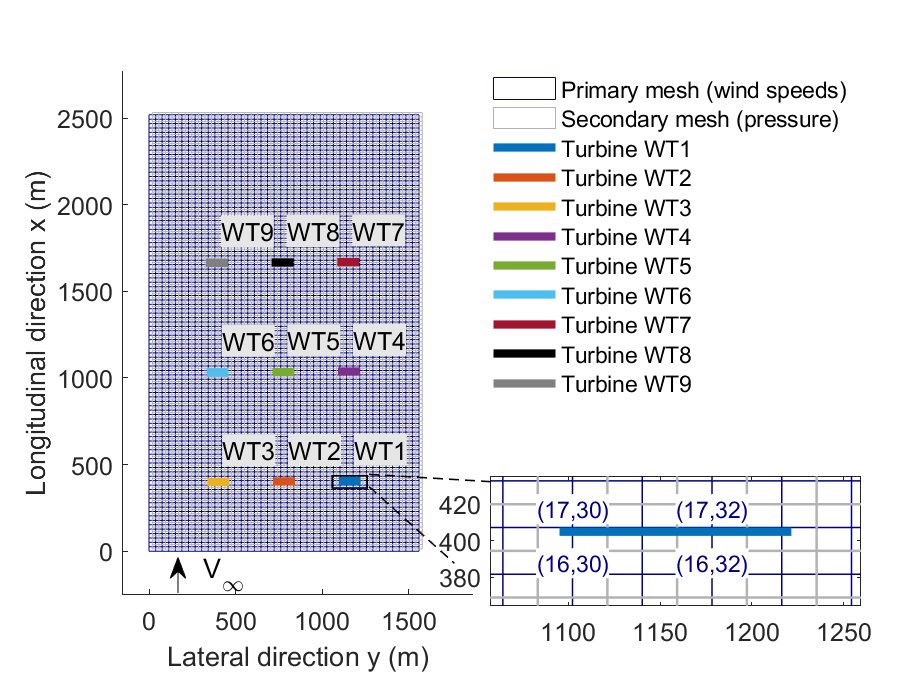
\includegraphics[width=0.85\textwidth,trim={0 0cm 0cm 0.0cm},clip]{figures/figDirETC/gridmesh9_tex.eps}
\caption[WFSim mesh setup for a nine-turbine wind farm.]{WFSim mesh setup for a nine-turbine wind farm. The primary mesh (blue) is used for wind speed calculations, and the secondary mesh (gray) for pressure. Turbines are shown as colored bars. Zoomed-in area around WT1 shows primary grid point indices.} 
\label{fig:9TurbMesh}
\end{figure}
The turbine locations for the default nine-turbine wind farm layout included with WFSim are depicted as bold, colored lines. The figure shows the entire wind field area and highlights a zoom around the first turbine, showing that the nodes of the secondary grid correspond to the centers of the primary grid cells and providing the index pair of the node as blue numbers. The effective wind speeds of the turbines is calculated based on the wind speeds at the nodes of the primary grid in front of the turbines. In the example in Figure~\ref{fig:9TurbMesh} these grid points leveraged for upstream wind turbine WT1 are the points in the 16$^{\text{th}}$ row from the 30$^{\text{th}}$ to the 33$^{\text{rd}}$ column. For better readability, only every second mesh point is annotated with the corresponding grid index in the zoom on the turbine location.

The finite volume method discretizes Partial Differential Equations (PDEs) such as the NSE by integrating them over small control areas to ensure the conservation of fluxes, such as the air mass flowing through the wind farm, across cell boundaries. In the WFSim 2D simulation, pressure is stored at the center of each grid cell, corresponding to the mesh points of the secondary mesh, while the longitudinal wind speed $v_x$, acting in vertical direction, is stored at the top and bottom edges and the lateral wind speed $v_y$ is stored at the left and right edges of the primary mesh.

In CFD software, the convective terms from Equation~\eqref{eq:NSE2d} are approximated with a combination of differencing schemes. These schemes compute how the wind carries momentum across the grid by switching between approaches to balance numerical stability and solution accuracy. Upstream differencing, which is more stable, is used when wind speeds are high, whereas central differencing, which is more accurate, is employed when wind speeds are low. Temporal discretization is performed using an implicit Euler method.

Numerical cost varies considerably with grid resolution, timestep, and available computing resources; for example, NREL's SOWFA documentation \cite{churchfield2012overview} reports a coarse LES example that ran at approximately 1.6\,s of wall-clock time per 1\,s of simulated time on 32 cores. Wall-clock time is the total real-world time elapsed from the start to the end of a simulation, including computation, inter-processor communication, disk I/O, memory access, and any idle or waiting time.

In \cite{boersma2018control}, which introduces the WFSim software, a mean computation time of approximately 0.02\,s per 1\,s timestep is reported on a single-core Intel~i7 platform instead on a server cluster. While no direct wall-clock time comparison with SOWFA is provided, the paper notes that high-fidelity LES solvers such as SOWFA require orders-of-magnitude longer runtimes and substantially more computational resources. In a two-turbine test case, WFSim was shown to reproduce the center-line mean wake velocity and power output time series from SOWFA reasonably well.

In WFSim, the wind field is approximated by a linear system for the velocity and pressure fields at each timestep, resulting in a significant reduction in simulation time and required computing resources. A more detailed overview of WFSim, including equations, is provided in Section~\ref{sec:WindFarmSimulationWFSim}, which also discusses the modifications made to WFSim to obtain the simulation results in \cite{dittmer2022data,dittmer2023koopman}.

\subsection{Wind Farm Control}\label{Subsection:Windfarmcontrol}
In this thesis, WFSim is used as a proof of concept for applying Koopman models to wind farm control, as it natively includes a farm-level controller that manages both turbine yaw $\gamma$ and thrust control $C_T^{\prime}$. The thrust controls, controlling the energy amount harvested by a turbine, are fictitious inputs used as substitutes for generator torque and blade pitch to avoid the need for a complex turbine model.

For closed-loop wind farm control, turbine control inputs are set to minimize the power reference tracking error and actuator activity, given a wind farm layout, a power grid reference $P_{\text{ref}}$, and the freestream wind speed $V_{\infty}$. Figure \ref{figBlockDiagramFarm} presents a block diagram of the control strategy for a wind farm consisting of two wind turbines.

\begin{figure}[ht]
\centering
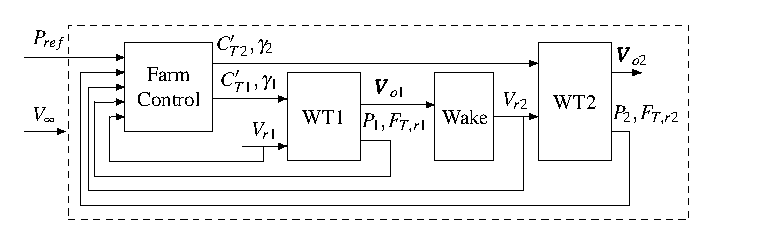
\includegraphics[width=0.8\textwidth,trim={0 0cm 0cm 0.3cm},clip]{figures/figDirETC/farmCtrl10_PandUr.pdf}
\caption{Block diagram of closed-loop wind farm control in WFSim}
\label{figBlockDiagramFarm}
\end{figure}

The wind farm layout and turbine parameters used in this study are consistent with those in \cite{sharan2022Koopman}, \cite{dittmer2022data}, and \cite{dittmer2023koopman}, upon which this thesis is based. The thrust control, which governs the amount of energy harvested by a turbine, is modeled as a fictitious input that substitutes for generator torque and blade pitch. This simplification eliminates the need for a detailed turbine model.

In the MPC implementation included with WFSim, it is assumed that the effective wind speeds at both turbines, $V_{r1}$ and $V_{r2}$, can be measured. These wind speeds, along with the power outputs $P_1$ and $P_2$, and the thrust forces $F_{T,r1}$ and $F_{T,r2}$, serve as feedback for the wind farm controller.

The effective wind speed $V_{ri}$ at the $i^{\text{th}}$ turbine is calculated as the root mean square of the wind speeds across the $n_r$ rotor segments:

\begin{align} \label{eqEffWindSpdWT}
V_{ri}(\gamma_{i}) &= \cos(\gamma_{i}) \sqrt{\frac{1}{n_r} \sum_{j = 1}^{n_r} V_{lj}^2},  
\quad  V_{lj}^2 = v_{xlj}^2 + v_{ylj}^2,
\end{align}
where $v_{xlj}$ and $v_{ylj}$ are the wind speed components in the $x$ and $y$ directions, respectively, at the $(l,j)$ grid point in the simulated WFSim domain. The vectors of wind speeds at the grid points directly behind the two turbines are denoted by $\bm{V}_{o1}$ and $\bm{V}_{o2}$.

Since the effective wind speed $V_{r2}$ is influenced by the wake of the first turbine, propagating through the wind speeds contained in $\bm{V}_{o1}$, the power and thrust output of the second turbine are also affected by the control input of the first turbine. 

The WFSim MPC discrete-time turbine model is given by:
\begin{align} \label{eqPowerWT}
\begin{split}
P_{i}(k+1) &= (1 - \tau) P_{i}(k) + \tau \frac{1}{2} \rho_a A_r \left(V_{ri}(\gamma_{i}(k))\right)^3 C_{Ti}^\prime(k), \\
F_{T,ri}(k+1) &= (1 - \tau) F_{T,ri}(k) + \tau \frac{1}{2} \rho_a A_r \left(V_{ri}(\gamma_{i}(k))\right)^2 C_{Ti}^\prime(k), \\
\hat{C}_{Ti}^\prime(k+1) &= (1 - \tau) \hat{C}_{Ti}^\prime(k) + \tau C_{Ti}^\prime(k),
\end{split}
\end{align}
with discrete sample time index $k$ and the constant $\tau$ as a discrete-time filter coefficient that determines the weighting between the current state and the new input at each time step. Larger values of  $\tau$ lead to faster updates. The state vector is defined as $\bm{x}_{\text{WT},i} = [P_i \;\; F_{T,ri} \;\; \hat{C}_{Ti}^\prime]^T$, where $P_i$ is the power and $F_{T,ri}$ is the thrust force of the $i^{\text{th}}$ turbine. The third state $\hat{C}_{Ti}^\prime$ is the filtered thrust control signal.

Equation~\eqref{eqPowerWT} is reformulated as
\begin{align} \label{eqWTWFSim}
\bm{x}_{\text{WT}i}(k+1) =\bm{A}_{\text{WT}i} \bm{x}_{\text{WT}i}(k) +\bm{B}_{\text{WT}i}(V_{ri}(\gamma_i))C_{Ti}^\prime(k), 
\end{align}
with the system and input matrices
\begin{align*}
\bm{A}_{\text{WTi}} = (1-\tau)\bm{I}_{3\times3},\text{ }\bm{B}_{\text{WTi}} = \tau[ C_P(V_{ri}(\gamma_i(k))) \quad C_F(V_{ri}(\gamma_i)) \quad 1]^T
\end{align*}
where $C_P(V_{ri}(\gamma_i)) = 1/2 \rho_a A_r (V_{ri}(\gamma_{i}))^3$ and $C_F(V_{ri}(\gamma_i)) = 1/2 \rho_a A_r (V_{ri}(\gamma_{i}))^2$ .
A concatenation into a wind farm model, with wind vector $\bm{V_r}$ and thrust $\bm{C}_{T}^\prime$ and yaw $\bm{\gamma}$ of all turbines, gives 
\begin{align} \label{eqLinWF}
\bm{x}_{\text{WF}}(k+1) = \bm{A}_{\text{WF}} \bm{x}_{\text{WF}}(k) + \bm{B}_{\text{WF}}(\bm{V_r}(\bm{\gamma}(k))) \bm{C}_{T}^\prime (k).
\end{align}
It is defined by the block diagonal system and input matrices $\bm{A}_{\text{WF}} \in {\mathbb{R}}^{3n_{\text{WT}} \times 3n_{\text{WT}}}$ and $\bm{B}_{\text{WF}} \in {\mathbb{R}}^{3n_{\text{WT}} \times n_{\text{WT}}}$ with turbine system and input matrices on their diagonals, and farm state $\bm{x}_{\text{WF}} \in {\mathbb{R}}^{3n_{\text{WT}}}$ for a farm with $n_{\text{WT}}$ turbines.

The models presented in Equations~\eqref{eqWTWFSim} and \eqref{eqLinWF} form the foundation of the wind farm baseline MPC algorithm and the qLMPC presented in this thesis. The theoretical frameworks required to design and implement MPC algorithms are introduced in Section~\ref{sec:Control-Theoretic Background}.

\section{Control-Theoretic Background}\label{sec:Control-Theoretic Background}
The following sections introduce the two modeling frameworks applied in this thesis, where first-principle based qLPV models are used to model wind turbines and Koopman theory based data-driven models for wind farms. This is followed by the MPC framework applied to both turbines and farms.

\subsection{Quasi-Linear Parameter-Varying Models}
\label{sec:qLPVmodels}

As described above, wind turbine dynamics are characterized by nonlinearities due to aerodynamic and structural effects. To be able to leverage the existing extensive linear control and estimation frameworks, Linear Parameter-Varying (LPV) and its generalized form, quasi-LPV (qLPV), can be used to represent nonlinear dynamics through a linear structure with time-varying parameters \cite{hoffmann2014survey}. These scheduling parameters capture the nonlinearity while preserving computational efficiency and physical interpretability. In the context of wind energy conversion systems, qLPV modeling enables systematic controller design across the whole operating range of a turbine without requiring full nonlinear computations at each time step.

\subsubsection{Standard and Velocity-based qLPV Models}
\label{sec:qLPVmodelTheory}

In general, nonlinear continuous-time dynamics can be expressed as
\begin{align} \label{eq:stateSpaceGeneral}
    \dot{\bm{x}}(t) = \bm{f}(\bm{x}, \bm{w}), \quad
    \bm{y}(t) = \bm{h}(\bm{x}, \bm{w}),
\end{align}
with the state $\bm{x} \in \mathbb{R}^{n_x}$, input $\bm{w} \in \mathbb{R}^{n_w}$, and output $\bm{y} \in \mathbb{R}^{n_y}$. The functions $\bm{f}$ and $\bm{h}$ are nonlinear, but locally smooth in the neighborhood of operating points.

The matrices of the LPV model are the linearization of Equation~\eqref{eq:stateSpaceGeneral} around relevant operating points, yielding the Jacobian-based matrices
\begin{equation}\label{eq:contMatricesqLPV}
    \begin{aligned}
        \bm{A}_c(\bm{x},\bm{w}) &= \nabla_{\bm{x}} \bm{f}(\bm{x},\bm{w}) \in \mathbb{R}^{n_x \times n_x}, \quad
        \bm{B}_c(\bm{x},\bm{w}) = \nabla_{\bm{w}} \bm{f}(\bm{x},\bm{w}) \in \mathbb{R}^{n_x \times n_u}, \\
        \bm{C}_c(\bm{x},\bm{w}) &= \nabla_{\bm{x}} \bm{h}(\bm{x},\bm{w}) \in \mathbb{R}^{n_y \times n_x}, \quad
        \bm{D}_c(\bm{x},\bm{w}) = \nabla_{\bm{w}} \bm{h}(\bm{x},\bm{w})\in \mathbb{R}^{n_y \times n_u}.
    \end{aligned}
\end{equation}
The scheduling parameter vector $\bm{\rho}_\Rho$ is constructed from selected states and inputs, and the qLPV model becomes:
\begin{equation} \label{eq:standardqLPV1}
    \begin{aligned}
        \dot{\bm{x}}(t) &= \bm{A}_c(\bm{\rho}_\Rho) \bm{x}(t) + \bm{B}_c(\bm{\rho}_\Rho) \bm{w}(t), \\
        \bm{y}(t) &= \bm{C}_c(\bm{\rho}_\Rho) \bm{x}(t) + \bm{D}_c(\bm{\rho}_\Rho) \bm{w}(t). 
    \end{aligned}
\end{equation}
An alternative, velocity-based qLPV formulation considers the derivatives of state and input rather than the states and inputs themselves \cite{cisneros2016efficient}. Differentiating Equation~\eqref{eq:standardqLPV1} gives:
%\begin{equation}\label{eq:velocityForm}
\begin{align*}
    \ddot{\bm{x}}(t) &= \bm{A}_c(\bm{\rho}_\Rho) \dot{\bm{x}}(t) +\bm{B}_c(\bm{\rho}_\Rho) \dot{\bm{w}}(t), \\
    \dot{\bm{y}}(t) &= \bm{C}_c(\bm{\rho}_\Rho)  \dot{\bm{x}}(t) + \bm{D}_c(\bm{\rho}_\Rho) \dot{\bm{w}}(t).
\end{align*}
%\end{equation}
This velocity-based form has the advantage of steady-state behavior at the origin ($\dot{\bm{x}}=\dot{\bm{w}}=0$), eliminating the need to store equilibrium state and input vectors at each operating point. Therefore, no trimming calculations are required once a physical model is derived based on the nonlinear dynamics. 

The MPC implementations presented in this thesis are formulated in discrete time within a velocity-based qLPV framework. The matrices $\bm{A}_d\in \mathbb{R}^{n_x \times n_x}$ and $\bm{B}_d\in \mathbb{R}^{n_x \times n_u}$ of the discrete velocity form can be obtained via zero-order hold discretization from their continuous-time counterparts from Equation~\ref{eq:contMatricesqLPV}:
\begin{equation} \label{eq:zoh1}
    \begin{aligned}
        \bm{A}_d(\bm{\rho}_\Rho) &= e^{\bm{A}_c(\bm{\rho}_\Rho)T_s}, \\
        \bm{B}_d(\bm{\rho}_\Rho) &= \left( \int_0^{T_s} e^{\bm{A}_c(\bm{\rho}_\Rho)\tau} \, d\tau \right) \bm{B}_c(\bm{\rho}_\Rho),
    \end{aligned}
\end{equation}
with the sample time $T_s$. A velocity-based discrete state-space model can then be set up as:
\begin{align} \label{eq:velocityFormDisc}
    \Delta\bm{x}(k+1) = \bm{A}_d(\bm{\rho}_\Rho) \Delta\bm{x}(k) + \bm{B}_d(\bm{\rho}_\Rho) \Delta\bm{u}(k)
\end{align}
with $
\Delta\bm{x}(k) = \bm{x}(k) - \bm{x}(k-1) \text{ and } \Delta\bm{u}(k) = \bm{u}(k) - \bm{u}(k-1).$

A subset of states $\bm{x}_{\text{sel}} \in \mathbb{R}^{n_{\text{sel}}}$ is selected for explicit inclusion in the qLPV model's state vector, enabling direct constraints on these states within the MPC scheme. The discrete difference vector $\Delta\bm{x}(k)$ at time sample $k$ is augmented with the vector 
\begin{equation}  \label{eq:differenceSelectedFormDisc}
    \begin{aligned}
        \bm{x}_{\text{sel}}(k) &= \bm{x}_{\text{sel}}(k-1) + \Delta \bm{x}_{\text{sel}}(k) \\
        &=  \bm{x}_{\text{sel}}(k-1) +  \bm{A}_{d,\text{sel}}\Delta \bm{x}_{\text{sel}}(k-1) +  \bm{B}_{d,\text{sel}}\Delta \bm{u}_{\text{sel}}(k-1),        
    \end{aligned}
\end{equation}
with the matrices $\bm{A}_{d,\text{sel}} \in  \mathbb{R}^{n_{\text{sel}} \times n_x}$ and  $\bm{B}_{d,\text{sel}} \in  \mathbb{R}^{n_{\text{sel}} \times n_x}$ representing the rows of the state and input matrices corresponding to the selected states.
%
%
The resulting augmented state-space model with the expanded state vector $\bm{x}_{\text{ext}} =[\bm{x}_{\text{sel}}^T \; \; \Delta\bm{x}^T ]^T$ is derived based on the matrices used in Equation~\eqref{eq:velocityFormDisc} and ~\eqref{eq:differenceSelectedFormDisc}:
\begin{equation}\label{eq:discreteVelocityqLPV}
    \begin{aligned}
        \begin{bmatrix} \bm{x}_{\text{sel}}(k+1) \\ \Delta\bm{x}(k+1) \end{bmatrix} 
        &= \begin{bmatrix} \bm{I}_{n_{\text{sel}}} & \bm{A}_{d,\text{sel}}(\bm{\rho}_\Rho) \\ 
            \bm{0}_{n_x \times n_\text{sel}} & \bm{A}_d(\bm{\rho}_\Rho) 
        \end{bmatrix}
        \begin{bmatrix} \bm{x}_{\text{sel}}(k) \\ \Delta\bm{x}(k) \end{bmatrix}
        + \begin{bmatrix} \bm{B}_{d,\text{sel}}(\bm{\rho}_\Rho) \\ \bm{B}_d(\bm{\rho}_\Rho) \end{bmatrix} \Delta\bm{u}(k), \\
        y(k) &= \bm{x}_{\text{sel}}(k) = \begin{bmatrix} \bm{I}_{n_{\text{sel}}} & \bm{0}_{n_\text{sel} \times n_x} \end{bmatrix} 
        \begin{bmatrix} \bm{x}_{\text{sel}}(k) \\ \Delta\bm{x}(k) \end{bmatrix},
    \end{aligned}
\end{equation}
where both the selected states and the discrete differences of all states appear explicitly in the dynamics. 

This structured state expansion, necessary for velocity-based qLPV models used in constrained MPC algorithms, increases, and may even double, the state dimension. This complicates stability analysis and controller synthesis using robustness guarantees such as Linear Matrix Inequality (LMI) schemes. However, for the low-order MPC implementation presented here, the increased state dimension is not critical, and LMI-based robustness guarantees are not pursued.

If the scheduling parameter $\bm{\rho}_\Rho$ depends solely on exogenous variables (i.e., inputs and parameters), the system is strictly LPV. However, if $\bm{\rho}_\Rho$ depends additionally or purely on endogenous variables (i.e., system states), as in the wind turbine models discussed here, the resulting structure is a qLPV model. This distinction is important as the dependence on model states introduces implicit dependencies that must be accounted for during control design. Concretely in the case of qLPV models used for MPC, the scheduling parameter has to be fixed to specific values for all samples of the prediction horizon to calculate the prediction trajectory in dependence of the states, see~\cite{cisneros2016efficient}.

The qLPV framework approximates nonlinear dynamic systems by allowing the model matrices to vary smoothly over the operating range. This can be achieved in several ways, for example through precomputed local linearizations, data-driven identification, or first-principles models combined with physics-based lookup tables. In this work, a combination of first-principles models and physics-based lookup tables is used.


\subsubsection{qLPV Models based on BEM Models and Actuator Disk Models}
\label{sec:quasi-LPVTurbineModel}

For wind energy applications, the mapping from the disturbance input wind speed and the control inputs generator torque and pitch angle to turbine states, including, e.g., rotor speed and tower displacement, is obtained from the mathematical representations of wind turbine physics described in Section~\ref{windTurbineModel}. For a wind turbine model, two-dimensional lookup tables for thrust and torque, dependent on blade pitch, wind speed, and rotor speed, are derived from BEM models implemented in the FAST software. When these nonlinear aerodynamic relationships are combined with linearized tower and drivetrain dynamics, the overall model becomes a nonlinear ODE system that can be approximated locally as linear around each operating point. For the BEM-based turbine model, the scheduling vector
\[
\bm{\rho}_{\Rho,\text{WT}} = [V_\infty \quad \omega_r \quad \beta]^T, 
\]
which is based on wind speed, rotor speed, and blade pitch angle, represents the variations in aerodynamics. The qLPV matrices thus reflect that changes in these three parameters immediately shift the effective aerodynamic of the turbine. Chapter \ref{sec:WindTurbineqLPVModels} provides a detailed derivation of two qLPV wind turbine models, both based on lookup tables for thrust and torque coefficients generated using FAST. 

For farm level control, the actuator disk model provided in Section~\ref{windTurbineModel} includes the effective inflow wind speed of all turbines as a scheduling variable for all $n_{\text{WT}}$ wind turbines of a farm
\[
\bm{\rho}_{\Rho,\text{WF}} = [V_{r,1} \quad V_{r,2} \quad \ldots \quad V_{r,n_{\text{WT}}} ]^T. 
\]
This effective wind speed depends on both exogenous variables (ambient turbulence, upstream wakes) and endogenous system states (thrust and yaw angle of the turbines). Consequently, the scheduling map becomes partially state-dependent which is the defining feature of a qLPV model. 

By combining these qLPV representations with predictive control formulations, one can design MPC controllers that explicitly accommodate nonlinear aerodynamic effects while maintaining convex optimization structure. The qLPV wind farm model used in the MPC formulation implemented in WFSim (see Section~2.3.2) is a representative example.

\subsection{Koopman Theory for System Modeling} \label{sec:Koopman}

This section presents the principle of Koopman operators, followed by a description of the design of the Koopman matrix as a prediction scheme based on Koopman operators. The Koopman framework allows the representation of any finite-dimensional nonlinear system as an infinite-dimensional linear system. Extended Dynamic Mode Decomposition (EDMD) and Extended Input-Output DMD (EIODMD) are used in this work for finite matrix approximations of the infinite-dimensional Koopman operator. This thesis leverages notations and methods from \cite{arbabi2018data}, where a data-driven Koopman MPC framework for nonlinear PDEs was presented. The approach identifies a Koopman-linear model via EDMD to design a feedback controller, demonstrated on Burgers’ equation and NSE cavity flow. The latter example is particularly relevant to wind farm control, as both are governed by NSEs.

\subsubsection{Koopman Operator and Matrix}\label{KoopmanOperator}

The Koopman operator $\mathcal{K}$ provides a framework for transforming finite-dimensional nonlinear dynamics into an infinite-dimensional linear system. By approximating this operator with a finite-dimensional representation, the tools of linear system analysis and control theory can be directly applied to nonlinear systems. This approach was originally proposed in \cite{koopman1931hamiltonian}. For its application to controls see, e.g.,\cite{proctor2018generalizing}, or \cite{kaiser2020data}.

Consider a time-invariant, discrete-time autonomous nonlinear dynamical system with state
$\bm{x} \in \mathbb{R}^{n_{x}}$ and function $F:\mathbb{R}^{n_{x}} \to \mathbb{R}^{n_{x}}$ at sample time $k$:
\begin{equation}
\bm{x}(k+1) = F(\bm{x}(k)). \label{eq:nonLinSysKoop}
\end{equation}
The Koopman framework uses the evolution of functions of the state, instead of the evolution of the state $\bm{x}$, to describe nonlinear dynamics as a linear dynamical system. The functions of the states are referred to as observables. The infinite-dimensional observable $g_\infty(\bm{x})$ belongs to a Hilbert space $\mathcal{H}$ \footnote{A Hilbert space generalizes the concept of the Euclidean space to possibly infinite dimensions \cite{korda2018linear}.}, creating an infinite-dimensional lifted state:
\begin{equation}
\bm{\varphi}_\infty(k) = g_\infty(\bm{x}(k)).
\end{equation}
The linear, infinite-dimensional Koopman operator $\mathcal{K}: \mathcal{H} \to \mathcal{H}$ is defined by its action on these observables, propagating them forward in time:
\begin{equation} \label{eq:KoopmanUnforced}
\bm{\varphi}_\infty(k+1) = (\mathcal{K}g_\infty)(\bm{x}(k)) = g_\infty(F(\bm{x}(k))) = g_\infty(\bm{x}(k+1)).
\end{equation}
Figure~\ref{fig:koopman-diagram} visualizes the concept of a Koopman operator applied to an unforced nonlinear system, as described in Equations~\eqref{eq:nonLinSysKoop} to \eqref{eq:KoopmanUnforced}
\begin{figure}[htb]
\centering
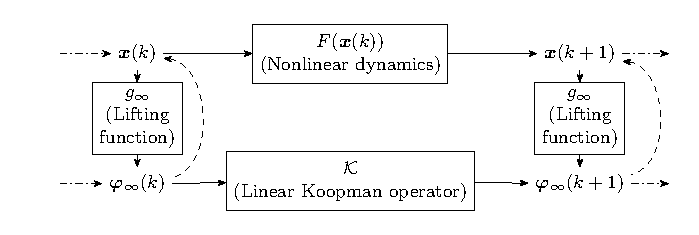
\includegraphics[width=0.82\textwidth, trim=0cm 0cm 0cm 0cm, clip]{figures/figuresBlockDiagram_IFAC23/KoopmanDiagram.pdf}
\caption{Block diagram of the nonlinear system, lifting function, and linear Koopman operator propagation for an unforced system (adapted from \cite{brunton2016koopman}).} 
\label{fig:koopman-diagram}
\end{figure}
The solid arrows show the main process flow. The dashed arcs indicate that the original states can be reconstructed from the lifted states and dash-dotted arrows represent the states' link to previous and future states.

Because the Koopman operator $\mathcal{K}$ is infinitely dimensional, it is generally impossible to use directly for real-time control calculations. This work hence employs a finite-dimensional approximation. A truncated lifting function $g: \mathbb{R}^{n_{x}} \to \mathbb{R}^{n_{g}}$ is used to create the approximated lifted state $\bm{\varphi} \in \mathbb{R}^{n_{g}}$:
\begin{equation}
\bm{\varphi}(k) = g(\bm{x}(k)). \label{eq:observ}
\end{equation}
By defining $g$ as a finite subset of $\mathcal{H}$, the operator $\mathcal{K}$ can be approximated by a finite-dimensional Koopman matrix $\hat{K}$. Note that in the following the truncated lifting functions and approximated lifted states are simply referred to as lifting function and lifted states, respectively, for better readability.

%
%Note that the finite function $g(\bm{x}(k))$ is an approximation of the observables $\g_\infty(\bm{x})$ which form a subset of an infinite-dimensional Hilbert space~$\mathcal{H}$, a complete vector space with an inner product that allows notions of length and angle to be defined. A Hilbert space generalizes the concept of the Euclidean space to possibly infinite dimensions \cite{korda2018linear}.% , providing a framework for analyzing functions and operators \cite{korda2018linear}.

%With lifting function $g$, the linear, infinite-dimensional Koopman operator $\mathcal{K}: \mathcal{H} \to \mathcal{H}$ for the nonlinear dynamical system is defined as
%\begin{equation} \label{eq:KoopmanUnforced}
%\bm{\varphi}(k+1) =(\mathcal{K}g)(\bm{x}(k)) = g(F(\bm{x}(k))) = g(\bm{x}(k+1)),
%\end{equation}
%where $\mathcal{K}$ propagates the observable $\bm{\varphi}(k) = g(\bm{x}(k))$ one time step forward. 


% Block diagram of the nonlinear system $F$, lifting function $g$, and linear Koopman operator $\mathcal{K}$ propagation for an unforced system (adapted from \cite{brunton2016koopman}).
% Block diagram of the Koopman operator framework. The top row depicts the nonlinear state evolution $F(\bm{x}(k))$, while the bottom row illustrates the linear evolution of the lifted observables $\boldsymbol{\varphi}(k)$ via the Koopman operator $\mathcal{K}$. 


This definition extends to nonlinear systems with input $\bm{w}$ as follows. The Koopman operator for controlled systems evolves on the extended state space $\mathbb{R}^{n_{x}} \times \ell(\mathcal{W})$, where $\ell(\mathcal{W})$ denotes the space of all infinite discrete input sequences $\bm{w} = (\bm{w}(k))_{k=1}^\infty$ \cite{arbabi2018data, korda2018linear}. The extended state vector 
\[
\bm{x}_w(k) = \begin{bmatrix} \bm{x}(k) \\ \bm{w}(k) \end{bmatrix} \in \mathbb{R}^{n_x + n_w}
\]
evolves according to the extended dynamics
\begin{align} \label{eq:KoopStateForced}
\bm{x}_w(k+1) = \tilde{F}_w(\bm{x}(k), \bm{w}(k)) = \begin{bmatrix} F_w(\bm{x}(k), \bm{w}(k)) \\ S(\bm{w}(k)) \end{bmatrix} = \begin{bmatrix} \bm{x}(k+1) \\ \bm{w}(k+1) \end{bmatrix},
\end{align}
where $F_w$ defines the state transition and the input sequence is moved forward by the shift operator $S$, defined by $S\left( (\bm{w}(k))_{k=1}^\infty \right) = (\bm{w}(k+1))_{k=1}^\infty$. The augmented flow map $\tilde{F}_w$ captures both the state transitions and the evolution of the exogenous signal.

The Koopman operator acts on the observables $\bm{\varphi}_w$ within the function space of the lifting function $g$. In practice, this infinite-dimensional operator is approximated by a finite-dimensional Koopman matrix 
\begin{align*}
\hat{\bm{K}} = [\bm{A}_K \;\; \bm{B}_K]
\end{align*}
This matrix maps the current extended lifted state to the next prediction:
\[
\bm{\varphi}(k+1) \approx \hat{\bm{K}} \bm{\varphi}_w(k) = [\bm{A}_K \;\; \bm{B}_K] \begin{bmatrix} \bm{\varphi}(k) \\ \bm{w}(k) \end{bmatrix},
\]
consistent with \cite{arbabi2018data, korda2018linear} and illustrated in Figure~\ref{fig:koopman-diagram-ext}. 
\begin{figure}[htbp]
\centering
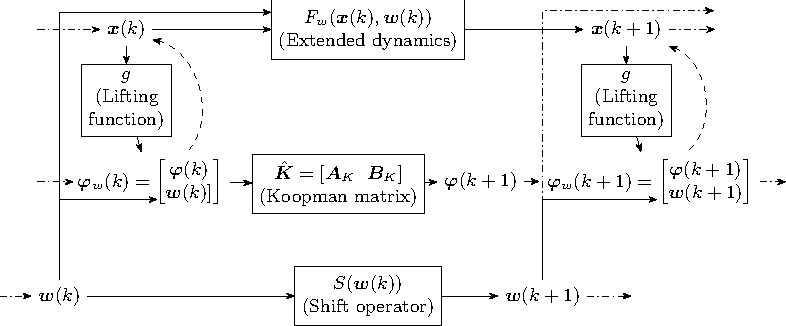
\includegraphics[width=0.95\textwidth, trim=0.cm 0.cm 0.cm 0cm, clip]{figures/figuresBlockDiagram_IFAC23/KoopmanDiagramExt.pdf}
\caption{Block diagram of the nonlinear system, approximated lifting function, shift operator, and Koopman matrix propagation for a forced system (adapted from \cite{proctor2018generalizing})}.
\label{fig:koopman-diagram-ext}
\end{figure}

This includes the extended state dynamics \(F_w\), the shift operator \(S\) acting on the input sequence, lifting functions \(g_w\) that map states and inputs to the extended, lifted observable space $\bm{\varphi}$, the Koopman matrix \(\hat{K}\) propagating lifted states and the lifted state at the next sample  $\bm{\varphi}(k+1)$ derived from the extended, lifted observable  $\bm{\varphi}_w(k)$. As before, dashed arrows indicate that the original states and inputs can be recovered from the lifted observables.

An illustrative example of lifting nonlinear dynamics into a higher-dimensional linear system is given in \cite{brunton2016koopman}. Consider the discrete-time nonlinear system
\begin{align} \label{eq:BruntonEx1}
x_1(k+1) &= \mu x_1(k), \\
x_2(k+1) &= \lambda x_2(k) - \lambda x_1^2(k) + u(k),
\end{align}
where \( x_1, x_2 \in \mathbb{R} \), \( \mu, \lambda \in \mathbb{R} \), and \( u \in \mathbb{R} \) is a scalar control input. The system is clearly nonlinear due to the \( x_1^2(k) \) term. By introducing a new observable \( \varphi(k) = x_1^2(k) \), the system can be rewritten as 
\begin{equation} \label{eq:BruntonEx2}
\varphi(k+1) = x_1^2(k+1) = \mu^2 x_1^2(k) = \mu^2 \varphi(k),
\end{equation}
which evolves linearly. Leveraging Equations~\eqref{eq:BruntonEx1} to~\eqref{eq:BruntonEx2} to stack the states and the observable into a lifted state vector, the dynamics can be expressed as a linear system:
\begin{equation}
\begin{bmatrix}
x_1(k+1) \\
x_2(k+1) \\
\varphi(k+1)
\end{bmatrix}
=
\begin{bmatrix}
\mu & 0 & 0 \\
0 & \lambda & -\lambda \\
0 & 0 & \mu^2
\end{bmatrix}
\begin{bmatrix}
x_1(k) \\
x_2(k) \\
\varphi(k)
\end{bmatrix}
+
\begin{bmatrix}
0 \\
1 \\
0
\end{bmatrix}
u(k).
\end{equation}
This construction yields a finite-dimensional linear representation of the original nonlinear system in lifted coordinates, where the Koopman operator corresponds to a matrix multiplication.

However, the Koopman operator cannot always be represented as a matrix multiplication. As shown in \cite{brunton2016koopman}, systems with multiple fixed points, periodic orbits, or attracting/repelling structures cannot be exactly represented by a finite-dimensional Koopman model, as  finite linear systems have a single equilibrium point only.
%In \cite{brunton2016koopman}, it is stated:
%\begin{quote}
%For any system with multiple fixed points, periodic orbits, or attracting/repelling structures, 
%there is no finite-dimensional Koopman invariant subspace that explicitly includes the state. 
%This follows from the fact that these systems cannot be topologically conjugate 
%to a finite-dimensional linear system with a single fixed point.
%\end{quote}
%In other words, any finite-dimensional linear system can only have one equilibrium point, 
%so it cannot exactly capture the behavior of more complex nonlinear systems.
As a discrete-time example where the Koopman operator is infinite-dimensional,  the scalar nonlinear system
\begin{equation}
x(k+1) = \mu x^2(k), \quad x \in \mathbb{R}, \ \mu \in \mathbb{R}
\end{equation}
is considered. Note that this system has two fixed points, concretely $x=0$ and $x=1/\mu$ for $\mu \neq 0$. The fixed point at the origin is attracting, since $f'(0)=0$, 
while the fixed point at $x=1/\mu$ is repelling, since $f'(1/\mu)=2$ with $|2|>1$. Defining the observable \( \varphi_1 = x^2 \) leads to
\begin{equation}
\varphi_1(k+1) = x^2(k+1) = (\mu x^2(k))^2 = \mu^2 x^4(k),
\end{equation}
which introduces the need for a new observable \( \varphi_2 = x^4 \). Continuing this process,
\begin{equation}
\varphi_2(k+1) = x^4(k+1) = (\mu x^2(k))^4 = \mu^4 x^8(k),
\end{equation}
and so on, yields an infinite sequence of new observables. Therefore, a finite-dimensional Koopman operator cannot capture the dynamics of this system. The lifted space is, in this example, infinite-dimensional.

In cases where the Koopman operator is infinite-dimensional, one approach is to approximate it with a finite matrix using a suitable set of observables. This Koopman matrix can be identified directly from data by DMD, without requiring a closed-form model of the underlying dynamics. This makes the approach applicable to wind farm control, where the flow and wake dynamics are governed by the Navier-Stokes equations, for which no general analytical solution is known and whose discretization yields a state dimension far too large for an analytical lifting.


\subsubsection{Koopman Matrix for Wind Farm Modeling}\label{KoopmanIdentification}

In this work, the system states of the MPC model used to calculate the optimal control inputs are the wind speeds acting on the turbines. For a qLMPC design, estimating the wind speeds based on a wind measurement in front of the upstream turbine, EDMD is used. For a linear Koopman MPC design, which uses an estimate of the power output of the turbines, EIODMD is applied.

The discrete-time nonlinear dynamical system can be extended by an output $\bm{y}$ as
\begin{equation}
\bm{x}(k+1) = F_w(\bm{x}(k), \bm{w}(k)), \quad 
\bm{y}(k) = G(\bm{x}(k), \bm{w}(k)) \label{eq:nonLinSys}
\end{equation}
with states $\bm{x} \in \mathbb{R}^{n_{x}}$, inputs $\bm{w} \in \mathbb{R}^{n_{w}}$, outputs $\bm{y} \in \mathbb{R}^{n_{y}}$, and nonlinear functions $F_w : \mathbb{R}^{n_{x}} \times \mathbb{R}^{n_{w}} \to \mathbb{R}^{n_{x}}$ and $G : \mathbb{R}^{n_{x}} \times \mathbb{R}^{n_{w}} \to \mathbb{R}^{n_{y}}$.


Lifting functions $g$ are defined as before as nonlinear combinations of the original states $\bm{x}$. In this work a new state $\bm{\varphi}\in\mathbb{R}^{n_{g}}$ is defined as a concatenation of the state $\bm{x}$ and the nonlinear combination of the states $g_{\varphi}$, i.e., the observables $\bm{\varphi}_g = g_{\varphi}(\bm{x})$, and hence $ \bm{\varphi} = g(\bm{x})$ with $\bm{\varphi}^T = [\bm{x}^T \; \bm{\varphi}_g^T]^T$.

A finite linear approximation of the nonlinear system given in Equation~\eqref{eq:nonLinSys} is:
\begin{align*}
\bm{\varphi}(k+1)=\bm{A}_{\hat{K}}\bm{\varphi}(k)+\bm{B}_{\hat{K}}\bm{w}(k), \quad 
\hat{\bm{y}}(k) = \bm{C}_{\hat{K}}\bm{\varphi}(k) + \bm{D}_{\hat{K}}\bm{w}(k),%\label{eq:linearPredictor}
\end{align*}
where $\hat{\bm{y}}$ is the vector of predicted output $\bm{y}$, $\bm{A}_{\hat{K}}\in \mathbb{R}^{{n_g}\times {n_g}}$, $\bm{B}_{\hat{K}}\in \mathbb{R}^{n_\varphi\times n_w}$, $\bm{C}_{\hat{K}}\in \mathbb{R}^{n_y\times n_\varphi}$, and $\bm{D}_{\hat{K}}\in \mathbb{R}^{n_y\times n_w}$.

For EIODMD, data from $n_o$ samples containing the measured state, input, and output vectors are collected and organized into two data matrices. The first matrix, $\bm{X}_{\text{EIODMD}}$, contains the state and input snapshots. The second matrix, $\bm{X}_{\text{EIODMD},+}$, contains the subsequent state snapshots and the corresponding outputs:
\begin{align} \label{eq:DataCollAIC}
\bm{X}_{\text{EIODMD}} &= \begin{bmatrix} 
\bm{x}(1) & \bm{x}(2) & \dots & \bm{x}(n_o-1) \\
\bm{w}(1) & \bm{w}(2) & \dots & \bm{w}(n_o-1)
\end{bmatrix} \in \mathbb{R}^{(n_x+n_w)\times (n_o-1)}, \\
\bm{X}_{\text{EIODMD},+} &= \begin{bmatrix} 
\bm{x}(2) & \bm{x}(3) & \dots & \bm{x}(n_o) \\
\bm{y}(1) & \bm{y}(2) & \dots & \bm{y}(n_o-1)
\end{bmatrix} \in \mathbb{R}^{(n_x+n_y)\times (n_o-1)}.
\end{align}
%
The matrices $\bm{A}_{\hat{K}}, \bm{B}_{\hat{K}}, \bm{C}_{\hat{K}}$, and $\bm{D}_{\hat{K}}$ can be obtained by solving the optimization problem:
\begin{equation}
\min_{\hat{K}} \sum_{k=1}^{n_{o}-1} \left\Vert \begin{bmatrix}
\bm{\varphi}(k+1)\\ \bm{y}(k)
\end{bmatrix} - \hat{K} \begin{bmatrix}
\bm{\varphi}(k)\\ \bm{w}(k)
\end{bmatrix} \right\Vert_{2}^{2} \label{eq:ApproxKalman}
\end{equation}
with the Koopman matrix defined as:
\begin{align*}
\hat{K} = \begin{bmatrix}
\bm{A}_{\hat{K}} & \bm{B}_{\hat{K}}\\ 
\bm{C}_{\hat{K}} & \bm{D}_{\hat{K}} 
\end{bmatrix} \in \mathbb{R}^{(n_g + n_y) \times (n_g + n_w)}.
\end{align*}
%
The lifting functions are applied to data from the matrices $\bm{X}_{\text{EIODMD}}$ and $\bm{X}_{\text{EIODMD},+}$ to construct two matrices containing these lifted states:
\begin{align}
\bm{L}_u &= \begin{bmatrix} 
\bm{\varphi}(1) & \cdots & \bm{\varphi}(n_{o}-1)\\
\bm{w}(1) & \cdots & \bm{w}(n_{o}-1) 
\end{bmatrix} \in \mathbb{R}^{(n_g + n_w) \times (n_o - 1)}, \\
\bm{L}_{+} &= \begin{bmatrix}
\bm{\varphi}(2) & \cdots & \bm{\varphi}(n_{o})\\
\bm{y}(1) & \cdots & \bm{y}(n_{o}-1)
\end{bmatrix} \in \mathbb{R}^{(n_g + n_y) \times (n_o - 1)}. \label{eq:Lplus}
\end{align}
%
The optimization problem \eqref{eq:ApproxKalman} is reformulated as:
\[
\min_{\hat{K}} \left\Vert \bm{L}_{+} - \hat{K} \bm{L}_u \right\Vert_{F}^{2},
\]
where \( \left\Vert \cdot \right\Vert_{F} \) denotes the Frobenius norm. The analytical solution to this linear least squares problem is:
\begin{align*}
\hat{K} = \bm{L}_{+} \bm{L}_u^{\dagger},
\end{align*}
where \( ^{\dagger} \) denotes the Moore–Penrose pseudoinverse. For EDMD, only the upper part of the Koopman matrix \( \hat{K} \), denoted as \( \hat{K}_u \), which contains the system and input matrices, is used:
\begin{align}
\hat{K}_u = \begin{bmatrix} \bm{A}_{\hat{K}} & \bm{B}_{\hat{K}} \end{bmatrix}.
\end{align}
This matrix can be derived from the following problem:
\begin{equation}
\min_{\hat{K}_u} \sum_{k=1}^{n_{o}-1} \left\Vert
\bm{\varphi}(k+1) - \hat{K}_u
\begin{bmatrix}
\bm{\varphi}(k)\\ \bm{w}_u(k)
\end{bmatrix}
\right\Vert_{2}^{2}
\label{eq:ApproxKalmanEDMD}
\end{equation}
with the corresponding solution:
\begin{align*}
\hat{K}_u = \bm{L}_{+,u} \bm{L}_u^{\dagger},
\end{align*}
where \( \bm{L}_{+,u} \) is the upper part of the matrix \( \bm{L}_{+} \), as defined in Equation~\eqref{eq:Lplus}, i.e., the concatenation of samples of the vector \( \bm{\varphi} \) at different time steps. The input is denoted \( \bm{w}_u \), as it differs from the input used for EIODMD.

Figure~\ref{fig:BlockEDMDEIODMD} shows the inputs and outputs of the EDMD and EIODMD models.
\begin{figure}[h]
\centering
\subfloat[EDMD]{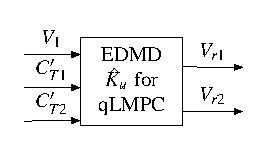
\includegraphics[width=0.35\textwidth]{figures/figuresBlockDiagram_IFAC23/farm1_OL2.pdf}}%
\hspace{0.05\textwidth}
\subfloat[EIODMD]{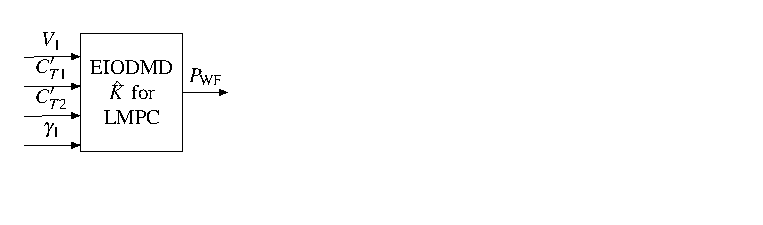
\includegraphics[width=0.35\textwidth, trim=0.0cm 1cm 8.5cm 0.5cm, clip]{figures/figuresBlockDiagram_IFAC23/EIODMD.pdf}}
\caption{Inputs and outputs of the EDMD and EIODMD models with lifted states $\bm{\varphi}$ based on effective wind speeds $V_{r1}$ and $V_{r2}$.}
\label{fig:BlockEDMDEIODMD}
\end{figure}

The states used to construct both models are the effective wind speeds acting on the turbines, specifically \( V_{r1} \) and \( V_{r2} \), along with lifted states derived from them. In this work, only polynomial functions are used, specifically the squares and cubes of the effective wind speeds, which correspond to aerodynamic force and power dependencies. The observable vector for both algorithms is:
\begin{align*}
\bm{\varphi} = [V_{r1} \quad V_{r2} \quad V^2_{r1} \quad V^2_{r2} \quad  V^3_{r1} \quad V^3_{r2}]^\top \in \mathbb{R}^6.
\end{align*}
For EDMD, the inputs include the thrust control inputs and the wind measurement taken in front of the first turbine. For EIODMD, the inputs include all those used in EDMD, as well as the yaw control input of the first turbine, since EIODMD is applied in a combined thrust and yaw control setting. Hence, the inputs are:
\begin{align*}
\bm{w}_{u} = [V_1 \quad C^{\prime}_{T1} \quad C^{\prime}_{T2}]^\top \in \mathbb{R}^3 \quad\text{and} \quad
\bm{w} = [V_1 \quad C^{\prime}_{T1} \quad C^{\prime}_{T2} \quad \gamma_1]^\top \in \mathbb{R}^4.
\end{align*}
The output of the EDMD model consists of the two states \( V_{r1} \) and \( V_{r2} \), whereas the output of the EIODMD model is the total wind farm power, i.e., the sum of the power outputs of both turbines.


While data-driven approaches such as EIODMD for Koopman MPC are particularly 
suitable for wind farm control, where complex wake interactions make first-principles 
modeling challenging, they may not be the optimal choice for individual wind turbines. 
The dynamics of a single turbine are well understood and can be accurately described 
using ODEs, making first principle-based control strategies more appropriate, with qLMPC being investigated in this work. 

%The following section explores the use of the qLPV framework, which leverages known turbine physics for efficient and reliable control design.

\subsection{Model Predictive Control}
Model Predictive Control (MPC) is an optimization-based control strategy that computes control inputs by repeatedly solving a finite-horizon optimal control problem online, see e.g. \cite{rawlings2017model} for a detailed description. At each discrete time step $k$, a sequence of future control inputs is determined by minimizing a cost function $J$ over a prediction horizon of $n_h$ steps, subject to the system dynamics and any state and input constraints. The general MPC problem takes the form:
\begin{align} \label{eqMPCGeneral}
    \begin{array}{l}
        \underset{\bm{U}(k)}{\text{min }} J(\bm{U}(k)) = \sum_{j=0}^{n_h - 1} \bm{x}(k+j)^T \bm{Q}\, \bm{x}(k+j) + \bm{u}(k+j)^T \bm{R}\, \bm{u}(k+j) \\
        \text{subject to } \bm{x}(k+j+1) = f(\bm{x}(k+j), \bm{u}(k+j)), \quad j \in \{0, 1, \dots, n_h-1\}
    \end{array}
\end{align}
where $\bm{x}$ and $\bm{u}$ denote the state and input vectors, $\bm{Q}$ and $\bm{R}$ are positive semi-definite weighting matrices penalizing state deviation and control effort, respectively. The vector $\bm{U}$ contains the values of the input vector at all samples of the prediction horizon and the vector $\bm{X}$ the corresponding state vectors:
\begin{align*}
     \bm{U}(k) &= \begin{bmatrix} \bm{u}(k)^T \quad \bm{u}(k+1)^T \quad \ldots \quad  \bm{u}(k+n_h-1)^T \end{bmatrix}^T \in \mathbb{R}^{n_h n_u \times 1},\\
      \bm{X}(k) &= \begin{bmatrix} \bm{x}(k)^T \quad \bm{x}(k+1)^T \quad \ldots \quad  \bm{x}(k+n_h-1)^T \end{bmatrix}^T \in \mathbb{R}^{n_h n_x \times 1}.
\end{align*}
%
 Only the first element of the optimal input sequence is applied, after which the horizon is shifted forward and the problem is solved again, following the receding horizon principle. Therefore, of the calculated values of the horizon only the first sample is directly used, but all values of the horizon of the current control input are stored to be used for a warm start in the next step.
 
The original formulation of MPC, as provided in Equation~\ref{eqMPCGeneral}, penalizes the amplitude of state and control values. The wind farm MPC controller, however, aims to minimize the power reference tracking error, instead of the states, as well as the actuator activity, instead of the actuator amplitude. Hence, the cost function $J$ is formulated based on the tracking error trajectory $\bm{E}(k)$ and the input trajectory $\Delta \bm{U}(k)$ for the $n_h$ sample steps of the prediction horizon:
\begin{align} \label{eqObjFun1}
    \begin{array}{l} 
        \underset{\bm{U}(k)}{\text{min }} J(\bm{U}(k)) = \bm{E}(k)^T \bm{Q}\bm{E}(k) +\Delta \bm{U}(k)^T \bm{R} \Delta \bm{U}(k) \\
        \text{subject to Equation } \eqref{eqLinWF}, \quad   k \in \{1, 2, \dots, n_h-1\}
    \end{array}
\end{align}
%
with the weighting matrices $\bm{Q}$ and $\bm{R}$. The trajectory of the farm power tracking error $\bm{E}$ is:
\begin{align*}
    \bm{E}(k) = \begin{bmatrix} e(k) & e(k+1) & \dots & e(k + n_h - 1) \end{bmatrix}^T \in \mathbb{R}^{n_h \times 1},
\end{align*}
where the power reference tracking error at time step $k$ on the farm level is calculated as 
\begin{align*}
    e(k) = P_{\text{ref}}(k) - P_{\text{WF}}(k). 
\end{align*}
%
The change in control inputs $\Delta \bm{U}$ is calculated as:
\begin{align*}
    \Delta \bm{U}(k) = \begin{bmatrix} \bm{u}(k) - \bm{u}(k-1) \\ \bm{u}(k+1) - \bm{u}(k) \\ \vdots \\ \bm{u}(k+n_h - 1) - \bm{u}(k + n_h - 2) \end{bmatrix} \in \mathbb{R}^{n_h n_u \times 1},
\end{align*}
with the vector $\bm{u}(k) \in \mathbb{R}^{n_u \times 1}$ containing all control inputs for all turbines at time~$k$.

This baseline MPC scheme is compared with Koopman-based MPC, i.e., an MPC based on a linear wind farm model derived using DMD. Koopman models are used to estimate the effective wind speeds rather than assuming that the measurements are available. To identify the Koopman models, known physical relationships of the NSEs are exploited when choosing the lifted states.

The next chapter describes in detail the set-up of two qLPV wind turbine models used for qLMPC for wind turbines. 
